\documentclass[11pt]{article}
\usepackage{amsmath,amssymb,amsthm}
\usepackage{mathtools}
\usepackage[margin=1in]{geometry}
\usepackage{tikz}
\usetikzlibrary{positioning,arrows.meta,decorations.pathreplacing}

\newtheorem{theorem}{Theorem}[section]
\newtheorem{lemma}[theorem]{Lemma}
\newtheorem{proposition}[theorem]{Proposition}
\newtheorem{corollary}[theorem]{Corollary}
\newtheorem{definition}[theorem]{Definition}
\newtheorem{remark}[theorem]{Remark}
\newtheorem{hypothesis}[theorem]{Hypothesis}

\newcommand{\Psurv}{\mathcal{P}_{\mathrm{surv}}}
\newcommand{\Sgood}{\mathcal{S}_{\mathrm{good}}}
\newcommand{\Ham}{\mathrm{HAM}}
\newcommand{\iface}{\mathrm{iface}}
\newcommand{\poly}{\mathrm{poly}}
\newcommand{\SIZE}{\mathrm{SIZE}}
\newcommand{\Ov}{\mathrm{Ov}}
\newcommand{\Vars}{\mathrm{Vars}}
\newcommand{\off}{\mathrm{off}}

\title{Hamiltonian Route: Separator Interface States\\
and the Anti-Stitch Framework}
\author{Joe Gallagher}
\date{March 18, 2026}

\begin{document}
\maketitle

\begin{abstract}
We prove that every Boolean fan-in-$2$ circuit computing the Hamiltonian Cycle
function $\mathrm{HAM}_n$ on $n$ vertices has size $2^{\Omega(n)}$.
The previous best lower bounds for explicit functions in NP were polynomial:
$\Omega(n^{3-o(1)})$ for formulas (H\r{a}stad~\cite{Hastad98}) and
$\Omega(n^{2.5-o(1)})$ via the Andreev function framework~\cite{Andreev87}.
Our proof combines three ingredients:
(i)~a separator-interface stitchability theory for Hamiltonian cycles,
exploiting the shared vertex set to avoid the isolation pathology
that kills the CLIQUE route;
(ii)~a \emph{multi-carrier funnel}: a recursive magnification scheme
maintaining $q = (\log n)^{O(1)}$ bichromatic carrier edges throughout
the recursion, where each step extends every carrier to a degree-visible
switch block, branches on all $2^q$ local-state patterns, and suppresses
the internal vertices---consuming the old carriers and replacing them with
new ones of the same restriction cost, so the background restriction mass
stays constant across the entire recursion depth, yielding an unconditional
$2^{\Omega(n)}$ formula lower bound;
(iii)~a legal monotone lift with continuation-packet sharing control,
extended to general circuits via a rooted-packet descent argument
that eliminates non-terminal packet-separating first escapes at
height $\ge 1$ and absorbs the unique terminal escape at height~$0$
into the occurrence-signature multiplicity bound.
\end{abstract}

\section{Motivation: Why Not CLIQUE}
\label{sec:why-not-clique}

The CLIQUE-based anti-stitch route fails for a structural reason.
The isolation lemma proves that for any
two distinct $k$-sets $S \neq T$, the mixed graph
$G_{S,T} = x_L^{(T)} \cup y_R^{(S)}$ contains no $k$-clique,
regardless of the $L/R$ edge partition.
This forces the frontier transcript map $m_S$ to be injective
on the packed family $\Psurv$ at \emph{every} frontier $S$.

Consequences:
\begin{enumerate}
\item The discrepancy indicator
  $D_e(T) := \mathbf{1}[m_S(T) \neq m_S(T^e)]$
  equals $1$ identically on the legal slice $L_e$
  (since $T \neq T^e$ and $m_S$ is injective).
\item The packed relevance graph
  $H_S^{\mathrm{pack}} \approx K_n$: every vertex swap
  is relevant.
\item $\nu(H_S^{\mathrm{pack}}) = \Theta(n)$, not polylog.
\item The control-set argument
  (Steps~5--8) requires $\nu \le \mathrm{polylog}(n)$ and
  therefore cannot produce a contradiction.
\item The entropy sweep requires $H(D_e) > 0$, but
  $D_e \equiv 1$ gives $H(D_e) = 0$.
\end{enumerate}

The root cause: $k$-sets differ in \emph{vertex membership},
and the isolation lemma exploits this to kill every mixed
graph.  Two different $k$-sets always produce distinguishable
frontier transcripts because their vertex-level differences
propagate through every $L/R$ partition.

\section{The Hamiltonian Pivot}
\label{sec:hamiltonian-pivot}

Hamiltonian cycles avoid this pathology.  Two Hamiltonian
cycles on $K_n$ use the \emph{same} vertex set $[n]$ and
differ only in edge selection.  Mixing the left edges of one
cycle with the right edges of another can produce a valid
Hamiltonian cycle --- the opposite of the CLIQUE isolation
property.

This means:
\begin{itemize}
\item $m_S$ is \emph{not} injective at every frontier:
  many cycles can share the same separator interface state.
\item $D_e$ is genuinely nonconstant: rerouting moves that
  do not change the separator interface give $D_e = 0$,
  while those that change it give $D_e = 1$.
\item The relevance graph is sparse (controlled by interface
  complexity, not by universal injectivity).
\item The entropy sweep has positive entropy to work with.
  (This motivates the Hamiltonian pivot; the main proof uses only
  the degree-visibility bias of $2$-opt moves, not the entropy
  sweep itself.)
\end{itemize}

The contradiction mechanism inverts:
\begin{center}
\begin{tabular}{lcc}
  & \textbf{CLIQUE} & \textbf{Hamiltonian} \\
\hline
Same transcript & fatal (no mixed clique)
  & \textbf{safe} (stitchable) \\
Different transcript, & --- & \textbf{fatal}
  (non-stitchable \\
\quad same circuit state & & \quad mixed input) \\
Transcript map & injective everywhere & non-injective \\
$D_e$ & $\equiv 1$ (degenerate) & nonconstant \\
$H(D_e)$ & $= 0$ & $> 0$ \\
Relevance graph & $\approx K_n$ & sparse \\
\end{tabular}
\end{center}


\section{Separator Interface State for Hamiltonian Cycles}
\label{sec:separator-state}

\subsection{Edge Partition and Boundary}

Fix a circuit $C$ of size $s$ computing $\Ham_n$
(Hamiltonian Cycle on $n$ vertices).
The input variables are edge indicators
$\{x_{\{i,j\}} : \{i,j\} \in \binom{[n]}{2}\}$.
Fix a topological ordering of the gates of $C$ and a
frontier position $S$.  Let
\[
  E_{\le S} := \{\text{edge variables queried before } S\},
  \qquad
  E_{> S} := \{\text{edge variables queried after } S\}.
\]
These partition $\binom{[n]}{2}$ into left and right edges.

\begin{definition}[Boundary vertices]
\label{def:boundary}
\[
  B_S := \{v \in [n] : v \text{ is incident to at least one
  edge in } E_{\le S} \text{ and at least one in } E_{> S}\}.
\]
\end{definition}

For a general balanced frontier, $|B_S|$ can range from
$\Theta(n)$ to $n$.  For the \emph{chromatic frontier}
$S_\chi$ used in the main proof (\S\ref{subsec:multi-carrier-funnel}),
every vertex $v$ has $\approx n/2$ monochromatic neighbours
(left edges) and $\approx n/2$ bichromatic neighbours (right edges),
so $|B_{S_\chi}| = n$.

\subsection{The Interface State}

\begin{definition}[Left partial subgraph]
For a Hamiltonian cycle $H$ on $[n]$, define
\[
  L_S(H) := H \cap E_{\le S}
\]
to be the subgraph of $H$ consisting of edges queried
before frontier $S$.
\end{definition}

Since $H$ is a 2-regular spanning subgraph of $K_n$,
every vertex $v$ has $\deg_H(v) = 2$.
In the partial subgraph $L_S(H)$, each vertex has
left-degree $0$, $1$, or $2$.  The connected components
of $L_S(H)$ are paths (for vertices with left-degree
$\le 1$ at their endpoints) or cycles (closed components
fully contained in $E_{\le S}$).

\begin{definition}[Hamiltonian separator interface state]
\label{def:interface-state}
For a Hamiltonian cycle $H$ and frontier $S$, define
\[
  \sigma_S(H) := \bigl(d_S(H),\; \pi_S(H),\; c_S(H)\bigr)
\]
where:
\begin{enumerate}
\item \textbf{Degree profile.}
  $d_S(H) : B_S \to \{0,1,2\}$,
  \[
    d_S(H)(v) := \deg_{L_S(H)}(v).
  \]
\item \textbf{Path-pairing.}
  Let
  \[
    U_S(H) := \{v \in B_S : d_S(H)(v) = 1\}
  \]
  be the set of boundary vertices with left-degree exactly
  $1$ (the ``dangling endpoints'').
  Since $L_S(H)$ consists of paths and cycles,
  $|U_S(H)|$ is even: each path-component with at least
  one edge contributes exactly two boundary endpoints of
  left-degree~$1$ (its two path-endpoints), so
  $|U_S(H)| = 2 \times (\text{number of such path-components})$.
  Define $\pi_S(H)$ to be the perfect matching on $U_S(H)$
  where $u \sim_{\pi_S(H)} v$ iff $u$ and $v$ are the two
  boundary endpoints of the same path-component of $L_S(H)$.
\item \textbf{Premature-cycle flag.}
  $c_S(H) \in \{0,1\}$, where $c_S(H) = 1$ iff $L_S(H)$
  contains a cycle component that is not the full
  Hamiltonian cycle $H$ itself.
\end{enumerate}
\end{definition}

\begin{definition}[Right partial subgraph and right pairing]
\label{def:right-pairing}
For a Hamiltonian cycle $H$ and frontier $S$, define the \emph{right partial subgraph}
\[
  R_S(H) := H \cap E_{>S}.
\]
The \emph{right pairing} $\rho_S(H)$ is the perfect matching on $U_S(H)$ where
$u \sim_{\rho_S(H)} v$ iff $u$ and $v$ are the two boundary endpoints of the same
path-component of $R_S(H)$.

\smallskip
\noindent\textit{Well-definedness.}
Every $u \in U_S(H)$ has $d_S(H)(u) = 1$, so $\deg_{L_S(H)}(u) = 1$ and hence
$\deg_{R_S(H)}(u) = \deg_H(u) - \deg_{L_S(H)}(u) = 2 - 1 = 1$.
Thus $u$ is an endpoint of exactly one path-component of $R_S(H)$.
The other endpoint of that path-component also has right-degree~$1$ in $R_S(H)$,
hence left-degree~$1$ in $L_S(H)$, hence lies in $U_S(H)$ as well.
This is the symmetric argument to Lemma~\ref{lem:normal-form}(2) applied to $R_S(H)$.
Therefore $\rho_S(H)$ is a well-defined perfect matching on $U_S(H)$.
\end{definition}

\begin{remark}
\label{rem:premature-cycle}
For an actual Hamiltonian cycle $H$ at a proper balanced interior
frontier $S$ (i.e.\ both $E_{\le S}$ and $E_{> S}$ are nonempty),
$c_S(H) = 0$ unconditionally, not merely generically.
Since $H$ is a single spanning cycle on $[n]$ and $S$ is proper,
$L_S(H)$ is a proper subgraph of $H$ and therefore cannot contain
$H$ itself as a component.  Any cycle component of $L_S(H)$ would
be a premature closed subtour: its vertices would have left-degree
$2$, leaving no degree budget for right-side $H$-edges, contradicting
$H$ being a spanning cycle using edges on both sides.
The flag is included only for closure under analysis of mixed or
invalid configurations that arise in the collision arguments.
\end{remark}


\section{Same-State Stitchability}
\label{sec:stitchability}

This is the foundational theorem replacing CLIQUE's
isolation lemma.  Where isolation made same-transcript
pairs \emph{fatal}, stitchability makes same-interface
pairs \emph{safe}.

\subsection{Path-Component Normal Form}

The connectivity argument for stitchability requires
knowing that the interface state $(d, \pi, c)$ fully
determines the boundary multigraph.  The following lemma
establishes this.

\begin{lemma}[Path-component normal form]
\label{lem:normal-form}
Let $H$ be a Hamiltonian cycle on $[n]$ and $S$ a
balanced interior frontier with $c_S(H) = 0$.  Then:
\begin{enumerate}
\item Every connected component of $L_S(H)$ is a simple
  path (possibly a single vertex).
\item Every path-component with at least one edge has
  exactly two endpoints of left-degree $1$.
  Both endpoints are boundary vertices (elements of
  $B_S$).
\item Internal vertices of a path-component (left-degree
  $2$) may or may not be boundary vertices; in either
  case they do not affect the boundary multigraph.
\item Isolated vertices (left-degree $0$) are boundary
  vertices iff they are incident to at least one edge
  on each side of the partition.
\item No connected component of $L_S(H)$ is disjoint
  from $B_S$ unless it is a single vertex with no
  left-side edges.
\item The boundary multigraph --- whose $L$-edges are the
  pairs $\{u,v\}$ for path-components with boundary
  endpoints $u, v$ --- is completely determined by
  $(d_S(H), \pi_S(H))$.
\end{enumerate}
\end{lemma}

\begin{proof}
\textbf{(1)} Since $c_S(H) = 0$, there are no cycle
components in $L_S(H)$ (other than possibly $H$ itself,
which only occurs at trivial frontiers where all $H$-edges
are left edges).
At any balanced interior frontier, at least one $H$-edge
is on each side, so no full-cycle component exists.
Therefore every component is a path.

\textbf{(2)} A path-component with at least one edge has
exactly two endpoints of degree~$1$ in $L_S(H)$.
Each such endpoint $v$ has $\deg_{L_S(H)}(v) = 1$, so $v$
uses one $H$-edge on the left side.  Since
$\deg_H(v) = 2$, the other $H$-edge incident to $v$ is on
the right side: $v$ is incident to at least one edge in
$E_{> S}$ (namely, this right $H$-edge).
Also, $v$ is incident to at least one edge in $E_{\le S}$
(its left $H$-edge).  Therefore $v \in B_S$.

\textbf{(3)} An internal vertex $w$ of a path-component
has $\deg_{L_S(H)}(w) = 2$: both its $H$-edges are left
edges.  It has no right $H$-edges, but it may still be
incident to non-$H$ edges on the right side
(from $K_n \setminus H$), making it a boundary vertex.
In the boundary multigraph, $w$ is contracted into its
path-component and does not contribute an endpoint.

\textbf{(4)} An isolated vertex $v$ has
$\deg_{L_S(H)}(v) = 0$: both $H$-edges are right edges.
So $v$ is incident to right-side edges (its $H$-edges).
At a balanced frontier, $v$ is also incident to left-side
edges (from $K_n$, since $|E_{\le S}| = \Theta(n^2)$ and
$v$ has degree $n-1$).  Hence $v \in B_S$ with
$d_S(H)(v) = 0$.

\textbf{(5)} Suppose a connected component $P$ of
$L_S(H)$ is disjoint from $B_S$.
If $P$ has an edge, its endpoints have left-degree $1$
and hence are boundary vertices by~(2) --- contradiction.
So $P$ must be a single isolated vertex $v$ with
$v \notin B_S$.  This means $v$ is incident only to
edges on one side.  Since $\deg_{L_S(H)}(v) = 0$, all
$H$-edges of $v$ are right edges, and the only way
$v \notin B_S$ is if $v$ has no left-side edges at all
--- which can only happen if every edge of $K_n$ incident
to $v$ is in $E_{> S}$.  Such vertices can exist at a
balanced frontier, but this does not affect the
conclusion: $P$ is a single isolated vertex with no
left-side edges, exactly as claimed.

\textbf{(6)} By~(2), the path-components with edges have
boundary endpoints determined by membership in $U_S(H)$
(the degree-$1$ boundary vertices) and their pairing
$\pi_S(H)$.  Each pair in $\pi_S(H)$ corresponds to
exactly one $L$-edge in the boundary multigraph.
Internal vertices and isolated vertices are contracted
or absent and do not affect the multigraph edge set.
Hence the $L$-edges of the boundary multigraph are
exactly the pairs of $\pi_S(H)$.
\end{proof}


\subsection{The Stitchability Theorem}

We first isolate the precise boundary-graph fact used in the proof.

\begin{lemma}[Boundary-component correspondence]\label{lem:boundary-component-correspondence}
Let $M$ be a spanning $2$-regular graph on $[n]$ written as
\[
M=L\cup R,
\]
where every connected component of $L$ is either
\begin{enumerate}
    \item a simple path whose endpoints lie in $B_S$, or
    \item an isolated vertex,
\end{enumerate}
and every connected component of $R$ is either
\begin{enumerate}
    \item a simple path whose endpoints lie in $B_S$, or
    \item an isolated vertex.
\end{enumerate}
Assume moreover that neither $L$ nor $R$ contains a cycle-component.

Define the boundary multigraph $G_\partial(M)$ on vertex set $B_S$ by:
\begin{itemize}
    \item for each path-component of $L$ with boundary endpoints $u,v\in B_S$, add one $L$-edge $\{u,v\}$;
    \item for each path-component of $R$ with boundary endpoints $u,v\in B_S$, add one $R$-edge $\{u,v\}$.
\end{itemize}
(Isolated vertices contribute no edges.)

Then the connected components of $M$ are in bijection with the connected components of $G_\partial(M)$. In particular,
\[
M \text{ is a single Hamiltonian cycle }
\iff
G_\partial(M)\text{ is connected.}
\]
\end{lemma}

\begin{proof}
Contract each nontrivial path-component of $L$ and of $R$ to a single edge joining its two boundary
endpoints. Since $L$ and $R$ contain no cycle-components, every non-isolated component contributes
exactly one such edge. Isolated vertices contribute nothing.

Let $\widetilde M$ be the quotient multigraph obtained from $M$ by performing all these contractions.
By construction, $\widetilde M$ has vertex set $B_S$, and its $L$-edges and $R$-edges are exactly those
used to define $G_\partial(M)$. Hence
\[
\widetilde M = G_\partial(M).
\]

It remains to check that connected components are preserved under the contraction. Each contracted
path-component is connected, so contracting it cannot merge two distinct connected components of $M$,
nor can it split one. Thus the connected components of $M$ are in bijection with those of
$\widetilde M=G_\partial(M)$.

Since $M$ is spanning and $2$-regular, each connected component of $M$ is a cycle. Therefore $M$
is a single Hamiltonian cycle if and only if it has exactly one connected component, equivalently
if and only if $G_\partial(M)$ is connected.
\end{proof}

\begin{theorem}[Same-state stitchability]\label{thm:stitchability}
Let $S$ be a balanced interior frontier and let $H$ and $H'$ be
Hamiltonian cycles on $[n]$ with
\[
\sigma_S(H)=\sigma_S(H').
\]
Let
\[
M := L_S(H') \cup R_S(H),
\qquad
R_S(H):=H\cap E_{>S}.
\]
Then $M$ is again a Hamiltonian cycle on $[n]$.
\end{theorem}

\begin{proof}
We prove first that every vertex has degree exactly $2$ in $M$, and then that $M$ is connected.

\medskip
\noindent
\textbf{Degree condition.}
Fix $v\in[n]$.

If $v\in B_S$, then equality of interface states gives
\[
d_S(H)(v)=d_S(H')(v),
\]
hence
\[
\deg_{L_S(H')}(v)=\deg_{L_S(H)}(v).
\]
Therefore
\[
\deg_M(v)
=
\deg_{L_S(H')}(v)+\deg_{R_S(H)}(v)
=
\deg_{L_S(H)}(v)+\deg_{R_S(H)}(v)
=
\deg_H(v)
=
2.
\]

If $v\notin B_S$, then all edges incident to $v$ lie on one side of the frontier.

\begin{itemize}
    \item If $v$ is left-only, then every edge of $H$ incident to $v$ lies in $E_{\le S}$, and likewise
    for $H'$. Hence
    \[
    \deg_{L_S(H')}(v)=2,\qquad \deg_{R_S(H)}(v)=0,
    \]
    so $\deg_M(v)=2$.

    \item If $v$ is right-only, then similarly
    \[
    \deg_{L_S(H')}(v)=0,\qquad \deg_{R_S(H)}(v)=2,
    \]
    so $\deg_M(v)=2$.
\end{itemize}

Thus $M$ is spanning and $2$-regular.

\medskip
\noindent
\textbf{Connectivity.}
Because $H$ and $H'$ are Hamiltonian cycles at a balanced interior frontier, their premature-cycle
flags vanish:
\[
c_S(H)=c_S(H')=0.
\]
By Lemma~\ref{lem:normal-form} applied to $H$ and $H'$, every connected component
of $L_S(H)$ and $L_S(H')$ is either a simple path with boundary endpoints or an isolated vertex,
and similarly every connected component of $R_S(H)$ is either a simple path with boundary endpoints
or an isolated vertex. In particular, neither $L_S(H')$ nor $R_S(H)$ contains a cycle-component.

Hence Lemma~\ref{lem:boundary-component-correspondence} applies to
\[
M=L_S(H')\cup R_S(H).
\]

Now form the boundary multigraphs. Since $\sigma_S(H)=\sigma_S(H')$, we have
\[
\pi_S(H)=\pi_S(H').
\]
Therefore the $L$-edges contributed by $L_S(H')$ are exactly the same as the $L$-edges contributed
by $L_S(H)$. The $R$-edges in both $G_\partial(M)$ and $G_\partial(H)$ come from the same right
partial graph $R_S(H)$. Consequently,
\[
G_\partial(M)=G_\partial(H).
\]

But $H=L_S(H)\cup R_S(H)$ is itself a Hamiltonian cycle, so by
Lemma~\ref{lem:boundary-component-correspondence}, $G_\partial(H)$ is connected. Hence
$G_\partial(M)$ is connected, and therefore $M$ is connected as well.

So $M$ is a connected spanning $2$-regular graph, i.e.\ a Hamiltonian cycle.
\end{proof}

\begin{remark}[Symmetric application of Lemma~\ref{lem:normal-form} to $R_S(H)$]
\label{rem:normal-form-right}
Lemma~\ref{lem:normal-form} is stated for $L_S(H)$, but the proof above applies it to $R_S(H)$
by symmetry: define $R_S(H) := H \cap E_{>S}$ and note that the right partial subgraph satisfies
the same structural properties (path and isolated-vertex components, no premature cycles) by the
identical argument with left and right exchanged.  In particular, $c_S^R(H) = 0$ for any
Hamiltonian cycle $H$ at a proper balanced interior frontier, by the same reasoning as
Remark~\ref{rem:premature-cycle}.
\end{remark}


\section{Different-State Collision Is Fatal}
\label{sec:collision}

\subsection{Frontier Transcript Map and the Rectangle Property}
\label{subsec:frontier-transcript}

\begin{definition}[Frontier transcript map]
\label{def:frontier-transcript}
Let $C$ be a Boolean circuit with a fixed topological ordering of its gates, and let $S$ be a
frontier position.  The \emph{frontier transcript} $m_S(H)$ of an input $H$ is the vector of
values of all gates whose output wire is used by at least one gate strictly to the right of $S$,
when $C$ is evaluated on input $H$.  Formally,
\[
  m_S(H) \;:=\; \bigl(g(H)\bigr)_{g \in \partial_S(C)},
\]
where $\partial_S(C)$ denotes the set of gates whose output crosses the frontier $S$.
\end{definition}

\begin{lemma}[Rectangle property]
\label{lem:rectangle-property}
If $m_S(H) = m_S(H')$, then
\[
  C\!\bigl(x_L^{(H')},\, x_R\bigr) \;=\; C\!\bigl(x_L^{(H)},\, x_R\bigr)
  \qquad \text{for all right inputs } x_R.
\]
\end{lemma}

\begin{proof}
The right subcircuit of $C$ (the subgraph of gates strictly to the right of $S$) receives as
input only the values of the frontier gates $\partial_S(C)$ together with the right-side input
variables $x_R$.  It does not see the left-side input variables $x_L$ directly.  Therefore, if
$m_S(H) = m_S(H')$, the right subcircuit receives identical inputs on both $H$ and $H'$ for any
fixed $x_R$, and hence produces the same output.
\end{proof}

\begin{remark}
\label{rem:rectangle-general-circuit}
For formulas (where the frontier is a subtree boundary and every gate output is used at most once),
the rectangle property is the standard communication-complexity fact.  For general circuits with
fan-out $> 1$, a gate's output may be used on both sides of a partition; the definition of
$m_S(H)$ above captures exactly the gates whose output crosses to the right, so the same
one-line proof applies.  The legal monotone lift
(Proposition~\ref{prop:legal-monotone-lift}) converts the original circuit $C$ to a monotone
circuit $C^\pm$ on the legal slice; the rectangle property for $C^\pm$ on that slice follows
from the same argument, since frontier compatibility
(Proposition~\ref{prop:legal-frontier-compatibility}) ensures that $m_S^{\pm}$ is well-defined
on the legal slice.
\end{remark}

The error mechanism has two cases of different strength.
The degree-profile case is unconditional.  The
pairing-mismatch case requires an explicit witness
construction.

\subsection{Degree-Profile Collision}

\begin{theorem}[Degree-profile collision forces circuit
error]
\label{thm:degree-collision}
Let $C$ be a correct circuit for $\Ham_n$ with frontier
transcript map $m_S$.  If there exist Hamiltonian cycles
$H, H'$ with
\[
  m_S(H) = m_S(H')
  \qquad\text{but}\qquad
  d_S(H) \neq d_S(H'),
\]
then $C$ is incorrect on at least one input.
\end{theorem}

\begin{proof}
Since $m_S(H) = m_S(H')$, the rectangle property gives
$C(x_L^{(H')}, x_R) = C(x_L^{(H)}, x_R)$ for all $x_R$.
In particular,
\[
  C(x_L^{(H')}, x_R^{(H)})
  = C(x_L^{(H)}, x_R^{(H)}) = 1.
\]
But the mixed graph $M = L_S(H') \cup R_S(H)$ has
\[
  \deg_M(v) = d_S(H')(v) + (2 - d_S(H)(v))
\]
for every boundary vertex $v$.
Since $d_S(H) \neq d_S(H')$, there exists $v \in B_S$
with $d_S(H)(v) \neq d_S(H')(v)$, giving
$\deg_M(v) \neq 2$.
So $M$ is not $2$-regular, hence not a Hamiltonian cycle,
hence not even a union of cycles.
The circuit outputs $1$ on a non-Hamiltonian input.
Contradiction.
\end{proof}

\subsection{Pairing-Mismatch Collision}

\begin{definition}[Pairing overlay]
Let $U$ be a finite set of even cardinality. For perfect matchings $\pi$ and $\rho$ on $U$, the
\emph{overlay graph}
\[
O(\pi,\rho)
\]
is the multigraph on vertex set $U$ with edge set $\pi\cup\rho$. Since every vertex is incident to
exactly one $\pi$-edge and exactly one $\rho$-edge, $O(\pi,\rho)$ is $2$-regular, hence a disjoint
union of even cycles.
\end{definition}

\begin{lemma}[Exact count of one-cycle overlays]\label{lem:one-cycle-overlay-count}
Fix a perfect matching $\rho$ on a set $U$ of size $2t$ with $t\ge 2$. Then the number of perfect
matchings $\pi$ on $U$ such that $O(\pi,\rho)$ is a single cycle of length $2t$ is exactly
\[
2^{t-1}(t-1)!.
\]
\end{lemma}

\begin{proof}
Write the $\rho$-pairs as
\[
P_1,\dots,P_t,
\qquad
P_i=\{a_i,b_i\}.
\]

Suppose first that $O(\pi,\rho)$ is a single $2t$-cycle. Contract each $\rho$-edge $P_i$ to a single
supervertex $i$. Since the cycle alternates between $\rho$-edges and $\pi$-edges, after contraction
we obtain a simple cycle on the $t$ supervertices $\{1,\dots,t\}$.

Thus:
\begin{itemize}
    \item the overlay determines a cyclic ordering of the $t$ blocks $P_1,\dots,P_t$;
    \item for each adjacent pair of blocks in this cyclic order, one endpoint of the first block is
    matched by $\pi$ to one endpoint of the second block.
\end{itemize}

Conversely, given:
\begin{enumerate}
    \item a cyclic ordering of the $t$ blocks, and
    \item for each consecutive pair of blocks in that cyclic order, a choice of which endpoint of
    the first block is matched to which endpoint of the second,
\end{enumerate}
there is a unique perfect matching $\pi$ whose union with $\rho$ yields the corresponding alternating
$2t$-cycle.

Now count these choices.

\smallskip
\noindent
\emph{Step 1: cyclic order of the blocks.}
The number of cyclic orders of $t$ labeled blocks, modulo reversal, is
\[
\frac{(t-1)!}{2}\cdot 2 = (t-1)!,
\]
or more directly: fixing block $1$ as a root, the remaining $t-1$ blocks can be arranged around the
cycle in $(t-1)!$ ways.

\smallskip
\noindent
\emph{Step 2: endpoint choices.}
Fix the cyclic ordering. The alternating cycle enters block $P_1$ at one of its two endpoints;
fix this entry endpoint as a canonical root (say $a_1$). The cycle exits $P_1$ from $b_1$, and the
$\pi$-edge connects $b_1$ to one of the two endpoints of the next block $P_2$: this is a binary
choice. Once the entry endpoint of $P_2$ is determined, the exit endpoint is forced (it is the other
element of the pair), and the $\pi$-edge to $P_3$ again offers a binary choice. Continuing around the
cycle, each of the $t-1$ transitions from $P_2$ through $P_t$ contributes one independent binary
choice. (The transition from $P_t$ back to $P_1$ is forced, since the entry endpoint of $P_1$ was
fixed as $a_1$.) This gives exactly
\[
2^{t-1}
\]
distinct endpoint-choice patterns.

Multiplying, we obtain
\[
2^{t-1}(t-1)!
\]
perfect matchings $\pi$ for which $O(\pi,\rho)$ is a single $2t$-cycle.
\end{proof}

\begin{lemma}[Pairing-mismatch witness]\label{lem:pairing-witness}
Let $S$ be a balanced frontier. Let $H$ be a Hamiltonian cycle, and let
\[
\rho:=\rho_S(H)
\]
be the right pairing on
\[
U:=U_S(H),
\qquad
|U|=2t\ge 4.
\]
Then the number of perfect matchings $\pi'$ on $U$ for which the overlay $O(\pi',\rho)$ is
\emph{disconnected} is exactly
\[
(2t-1)!! - 2^{t-1}(t-1)!.
\]
Equivalently, the proportion of perfect matchings producing a disconnected overlay is
\[
1-\frac{2^{t-1}(t-1)!}{(2t-1)!!}
=
1-\frac{2^{2t-1}t!(t-1)!}{(2t)!}.
\]
In particular,
\[
\frac{2^{t-1}(t-1)!}{(2t-1)!!}
=
\Theta(t^{1/2}2^{-t}),
\]
so
\[
(2t-1)!! - 2^{t-1}(t-1)!
=
(2t-1)!!\,(1-o(1)).
\]
\end{lemma}

\begin{proof}
The total number of perfect matchings on a $2t$-element set is $(2t-1)!!$. By
Lemma~\ref{lem:one-cycle-overlay-count}, exactly $2^{t-1}(t-1)!$ of them produce an overlay that is
a single $2t$-cycle. Every other perfect matching produces a $2$-regular overlay with at least two
connected components. This gives the exact formula.

For the asymptotic, use
\[
(2t-1)!!=\frac{(2t)!}{2^t t!},
\]
so
\[
\frac{2^{t-1}(t-1)!}{(2t-1)!!}
=
\frac{2^{2t-1}t!(t-1)!}{(2t)!}.
\]
Stirling's formula yields
\[
\frac{2^{2t-1}t!(t-1)!}{(2t)!}
=
\Theta(t^{1/2}2^{-t}),
\]
which tends to $0$ exponentially in $t$. Therefore the disconnected proportion is $1-o(1)$.
\end{proof}

\begin{corollary}[Pairing-mismatch collision forces circuit error]\label{cor:pairing-collision}
Let $S$ be a balanced frontier and let $H$ be a Hamiltonian cycle with
\[
|U_S(H)|=2t\ge 4.
\]
Let $H'$ be a Hamiltonian cycle satisfying
\[
d_S(H')=d_S(H),\qquad c_S(H')=c_S(H)=0,
\]
and assume that
\[
O(\pi_S(H'),\rho_S(H))
\]
has more than one connected component. Then the mixed graph
\[
M:=L_S(H')\cup R_S(H)
\]
is $2$-regular but not connected, hence is not a Hamiltonian cycle.

If, in addition,
\[
m_S(H')=m_S(H),
\]
then the circuit errs on the mixed input.
\end{corollary}

\begin{proof}
Because the degree profiles agree, the degree computation from
Theorem~\ref{thm:stitchability} shows that every vertex has degree $2$ in $M$.

As in the proof of Theorem~\ref{thm:stitchability}, the connected components of $M$ are in
bijection with the connected components of the boundary multigraph $G_\partial(M)$. The $L$-edges of
$G_\partial(M)$ are exactly the pairs of $\pi_S(H')$, and the $R$-edges are exactly the pairs of
$\rho_S(H)$. Therefore
\[
G_\partial(M)=O(\pi_S(H'),\rho_S(H)).
\]
If this overlay has more than one connected component, then $M$ has more than one connected component.
Since $M$ is spanning and $2$-regular, it is a disjoint union of at least two cycles, and hence is
not Hamiltonian.

If also $m_S(H')=m_S(H)$, then by the rectangle property the circuit outputs
\[
C(x^{(H')}_L,x^{(H)}_R)=C(x^{(H)}_L,x^{(H)}_R)=1
\]
on the mixed input, while the mixed graph is not Hamiltonian. Thus the circuit errs.
\end{proof}


% [Section on Interface State Counting removed: the martingale energy
%  framework is killed by the local switching involution's symmetry ---
%  the same involution that guarantees balanced state mass (H3) also
%  zeroes out the distributional leakage (H2), making delta=0 for every
%  atom.  The formula lower bound is now proved via the multi-carrier
%  funnel in the sweep section below.]


\section{The Multi-Carrier Amplification Program}
\label{sec:sweep}

This section develops the machinery for the exponential lower bound.
Before the definitions, we give a brief roadmap of the argument's
logical structure.

\paragraph{Proof roadmap.}
The goal is: every fan-in-$2$ circuit computing $\Ham_n$ has size
$2^{\Omega(n)}$.  The argument sandwiches a combinatorial quantity
$\Lambda(n)$ (the protocol-partition number) between a lower bound
independent of the circuit and an upper bound controlled by circuit
size.

\emph{Lower bound (independent of $C$).}
The multi-carrier funnel (\S\ref{subsec:multi-carrier-funnel})
recursively magnifies $\Lambda$ by a factor of $2^q$ per step, where
$q = (\log n)^A$ bichromatic carriers are maintained at each level.
Each step consumes and replaces all carriers, keeping the background
restriction mass constant.  After $\Theta(n/q)$ steps:
$\Lambda(n) \ge 2^{\Omega(n)}$.  This requires:
\begin{itemize}
\item the packed family is robust under polylog restrictions
  (Theorem~\ref{thm:packed-family}),
\item degree-visible $2$-opt moves exist in constant density
  (Lemma~\ref{lem:toggle-coupling},
   Theorem~\ref{thm:disjoint-switch-packing}),
\item $\Omega(n)$ disjoint switch blocks can be packed
  (Proposition~\ref{prop:consecutive-supply}), and
\item polylog-local contiguity gives positive probability that a
  uniform Hamiltonian cycle contains all carrier edges simultaneously
  (Lemma~\ref{lem:polylog-local-contiguity}).
\end{itemize}

\emph{Upper bound (from $C$).}
Given a circuit $C$ of size $s$, its legal monotone lift $C^{\pm}$
(\S\ref{subsec:width-to-size}) has size $\le 2s$.  The width-budget
proposition bounds $\Lambda(n) \le K |C^{\pm}| \mu_{\max}$, where
$\mu_{\max}$ is the maximum gate-sharing multiplicity across the
magnification tree.  The core technical work is bounding
$\mu_{\max} \le 2^{o(n)}$.

\emph{Multiplicity control.}
Continuation packets track how a single gate's evaluation propagates
across magnification levels.
The rooted-packet descent
(Theorem~\ref{thm:packet-separator-exclusion}) eliminates all
non-terminal packet-separating escapes by induction on rooted subtree
height; the unique terminal escape at height $0$ is absorbed into the
occurrence signature's terminal marker
(Definition~\ref{def:occurrence-signature}).  The signature
injectively encodes full branch histories using $O(1)$
corridor-lineage coordinates per level
(Lemma~\ref{lem:signature-injectivity}), and the codomain has size
$2^{o(n)}$ (Lemma~\ref{lem:signature-count}), giving
$\mu(g) \le 2^{o(n)}$ for every gate $g$
(Theorem~\ref{thm:subexp-multiplicity-pse}).

\emph{Sandwich.}
Combining: $2^{\Omega(n)} \le \Lambda(n) \le K \cdot 2s \cdot
2^{o(n)}$, so $s \ge 2^{\Omega(n)}$.

\medskip

The subsections below develop each piece in dependency order: packed
family robustness, degree-visibility bias, switch-block supply and
packing, multi-carrier funnel, formula lower bound, monotone lift,
continuation packets, packet-separator exclusion, and signature
rigidity.

\subsection{Packed Family}

\begin{theorem}[Packed family --- full Hamiltonian family]
\label{thm:packed-family}
Let $\mathcal{P}_n$ denote the set of all undirected
Hamiltonian cycles of $K_n$. Then:
\begin{enumerate}
\item \textbf{Density:}
$|\mathcal{P}_n| = (n-1)!/2 = 2^{\Theta(n \log n)}$.

\item \textbf{$2$-opt closure:}
$\mathcal{P}_n$ is trivially closed under every legal
$2$-opt move, since a legal $2$-opt move on a Hamiltonian
cycle of $K_n$ produces another Hamiltonian cycle of $K_n$.

\item \textbf{Robustness under polylog restrictions:}
For any consistent restriction $R = (F^+, F^-)$ with
$|F^+| + |F^-| \le (\log n)^a$,
\[
|\mathcal{P}_n(R)| = 2^{\Theta(n \log n)}.
\]
\end{enumerate}
\end{theorem}

\begin{proof}
\textbf{$2$-opt graph structure.}
The full $2$-opt graph on $\mathcal{P}_n$ is not just
connected: Fleischner--Hor\'ak--\v{S}ir\'a\v{n}~\cite{FHS07} proved it is
edge-Hamiltonian for every $n \ge 4$, so $\mathcal{P}_n$
comes with Gray-code-scale $2$-opt connectivity.

\textbf{Restriction robustness.}
Let $r := |F^+|$, $c :=$ the number of path-components
of $F^+$ (which must have max degree $\le 2$ and no
cycle-component for consistency).
Contract each path-component of $F^+$ to one supervertex.
This leaves $N = n - r$ objects. Each path-component can
be traversed in either orientation, giving a factor $2^c$.
The number of Hamiltonian cycles containing $F^+$ is
\[
|\mathcal{P}_n(F^+)| = 2^c \cdot \frac{(N-1)!}{2}
= 2^c \cdot \frac{(n - r - 1)!}{2}.
\]

Now impose the forbidden edges $F^-$. A fixed forbidden
edge appears in at most $2/(N-1)$ fraction of Hamiltonian
cycles on $N$ labeled objects after contraction. Hence
\[
|\mathcal{P}_n(R)| \ge |\mathcal{P}_n(F^+)|
\Bigl(1 - O\Bigl(\frac{|F^-|}{N}\Bigr)\Bigr).
\]
Since $r + |F^-| = (\log n)^a$,
$|\mathcal{P}_n(R)| = 2^{\Theta(n \log n)}$.
\end{proof}

\subsection{Rerouting Moves and the Degree-Change Criterion}

\begin{definition}[Separator-aware 2-opt rerouting]
\label{def:rerouting}
A \emph{rerouting move} $e$ at frontier $S$ is a local
modification of a Hamiltonian cycle $H$:
\[
  H \;\xmapsto{e}\; H^e
\]
where $H^e = (H \setminus \{ab, cd\}) \cup \{ac, bd\}$
for edges $ab, cd \in H$ and $ac, bd \notin H$, with
$a, b, c, d$ distinct, such that $H^e$ is again a
Hamiltonian cycle.

The \emph{discrepancy indicator} is
\[
  D_e(H) := \mathbf{1}[\sigma_S(H) \neq \sigma_S(H^e)].
\]
\end{definition}

\begin{lemma}[Degree-change criterion]
\label{lem:degree-change-criterion}
Let $e = (ab, cd \rightsquigarrow ac, bd)$ be a legal
$2$-opt move on $H$ at frontier $S$. Let
$\chi_S(f) \in \{L, R\}$ denote the side of edge $f$.
Then:
\[
d_S(H^e) = d_S(H) \quad\Longleftrightarrow\quad
\chi_S(ab) = \chi_S(ac) = \chi_S(cd) = \chi_S(bd).
\]
In particular, if the $4$-edge toggle set
$\{ab, ac, cd, bd\}$ is not monochromatic with respect
to the frontier partition, then
$\sigma_S(H^e) \neq \sigma_S(H)$ and $D_e(H) = 1$.
\end{lemma}

\begin{proof}
At the four touched vertices:
\begin{align*}
d_S(H^e)(a) - d_S(H)(a) &= \mathbf{1}_L(ac) - \mathbf{1}_L(ab), \\
d_S(H^e)(b) - d_S(H)(b) &= \mathbf{1}_L(bd) - \mathbf{1}_L(ab), \\
d_S(H^e)(c) - d_S(H)(c) &= \mathbf{1}_L(ac) - \mathbf{1}_L(cd), \\
d_S(H^e)(d) - d_S(H)(d) &= \mathbf{1}_L(bd) - \mathbf{1}_L(cd).
\end{align*}
All four vanish simultaneously iff
$\chi_S(ab) = \chi_S(ac) = \chi_S(cd) = \chi_S(bd)$.
A degree-profile change implies an interface-state change.
\end{proof}

\begin{definition}[Degree-visible 2-opt indicator]
\label{def:degree-visible}
For a legal $2$-opt move $e$ on $H$ at frontier $S$, define the
\emph{degree-discrepancy indicator}
\[
\Delta_e(H) := \mathbf{1}[d_S(H^e) \neq d_S(H)].
\]
By Lemma~\ref{lem:degree-change-criterion},
$\Delta_e(H) = 1$ iff the toggle set is not monochromatic.
\end{definition}

\begin{theorem}[Degree-visibility bias --- $C_4$ density model]
\label{thm:rerouting-relevance}
Let $S$ be a quasi-balanced frontier with left-edge density
\[
p_S := \frac{|E_{\le S}|}{\binom{n}{2}} = \frac{1}{2} + o(1).
\]
Let $H$ be uniform over $\mathcal{P}_n$ and $e$ be
chosen uniformly from the $n(n-3)/2$ legal $2$-opt moves
of $H$. Then:
\[
\Pr[D_e = 0] \in \Bigl[\frac{1}{8} - o(1),\;
\frac{1}{2} + o(1)\Bigr],
\qquad
\Pr[D_e = 1] \in \Bigl[\frac{1}{2} - o(1),\;
\frac{7}{8} + o(1)\Bigr],
\]
and therefore
\[
H(D_e) \ge h\!\left(\frac{1}{8}\right) - o(1) = \Omega(1).
\]
\end{theorem}

\begin{proof}
By Lemma~\ref{lem:degree-change-criterion}, $D_e = 0$
iff the $4$-edge toggle set $\{ab, ac, cd, bd\}$ is
monochromatic with respect to the frontier partition.
By Lemma~\ref{lem:toggle-coupling} (below),
\[
\Pr[D_e = 0] = t(C_4, G_L) + t(C_4, G_R) + O(1/n),
\]
where $G_L = ([n], E_{\le S})$, $G_R = ([n], E_{> S})$, and
$t(C_4, G)$ denotes the $C_4$-homomorphism density (the probability
that a uniformly random map $V(C_4) \to V(G)$ sends every
$C_4$-edge to a $G$-edge).

\textbf{Upper bound.}
For a graph of edge density $p$, the $C_4$-homomorphism
density is maximized asymptotically by the quasi-clique.
Since $C_4$ is a cycle, the Alon cycle-maximization fact
(cf.\ Blekherman--Patel) gives
\[
t(C_4, G_L) \le p_S^2 + o(1), \qquad
t(C_4, G_R) \le (1 - p_S)^2 + o(1).
\]
At $p_S = 1/2 + o(1)$:
$\Pr[D_e = 0] \le 1/2 + o(1)$.

\textbf{Lower bound.}
By Sidorenko's theorem for $C_4$
(cf.\ Bennett--Dudek--Lidick\'y--Pikhurko),
\[
t(C_4, G_L) \ge p_S^4 - o(1), \qquad
t(C_4, G_R) \ge (1 - p_S)^4 - o(1).
\]
At $p_S = 1/2 + o(1)$:
$\Pr[D_e = 0] \ge 1/8 - o(1)$.

\textbf{Entropy floor.}
Since $\Pr[D_e = 1] \in [1/2 - o(1),\; 7/8 + o(1)]$,
\[
H(D_e) \ge h(1/8) - o(1) = \Omega(1). \qedhere
\]
\end{proof}

\begin{lemma}[Toggle-vertex coupling]
\label{lem:toggle-coupling}
Let $H \sim \mathrm{Unif}(\mathcal{P}_n)$ and let $(a,b,c,d)$ be the
toggle vertices of a uniformly random legal $2$-opt move on $H$.  Let
$f : \binom{[n]}{4} \to [0,1]$ be any function of $4$-element subsets.
Then
\[
\bigl|\,\mathbb{E}[f(\{a,b,c,d\})]
- \mathbb{E}_{U}[f(U)]\,\bigr|
\;\le\; O(1/n) \cdot \|f\|_\infty,
\]
where $U$ is a uniform $4$-element subset of $[n]$.  In particular,
$\Pr[D_e = 0] = t(C_4, G_L) + t(C_4, G_R) + O(1/n)$
for the toggle set's monochromatic probability.
\end{lemma}

\begin{proof}
Write $H$ as the cyclic sequence $v_1$-$v_2$-$\cdots$-$v_n$-$v_1$.
A legal $2$-opt move selects positions $1 \le i < j \le n$ with
$j - i \ge 2$ and $j - i \le n - 2$ (non-adjacency), giving toggle
vertices $(v_i, v_{i+1}, v_j, v_{j+1})$.  There are exactly
$n(n{-}3)/2$ such pairs.

\emph{Step 1: per-tuple probability.}
For any fixed four distinct vertices $\{u_1, u_2, u_3, u_4\}$,
\[
\Pr[\text{$u_1$-$u_2$ and $u_3$-$u_4$ are non-adjacent edges of $H$}]
= \frac{2}{(n{-}1)(n{-}2)} - O(1/n^3).
\]
The main term: by Lemma~\ref{lem:polylog-local-contiguity} with
$\rho = \emptyset$ ($m = 0$), $e = 2$ edges in $c = 2$
path-components, the probability that $u_1u_2$ and $u_3u_4$ are both
edges of $H$ is $2^2 \cdot (n{-}3)!/(n{-}1)! \cdot (1 + O(1/n))
= 4/((n{-}1)(n{-}2)) \cdot (1 + O(1/n))$.  Dividing by $2$ for the
unordered edge-pair convention gives $2/((n{-}1)(n{-}2)) + O(1/n^3)$.
The $O(1/n^3)$ correction subtracts adjacent configurations: each of
the $n$ cycle edges has exactly $2$ adjacent edges, giving $n$ adjacent
pairs, each contributing $O(1/n^4)$ to the probability.

\emph{Step 2: TV distance.}
The toggle-vertex marginal $\mu_T$ assigns mass
$p_T(\{u_1,\ldots,u_4\})
= [2/((n{-}1)(n{-}2)) - O(1/n^3)] \cdot 3 / [n(n{-}3)/2]$
to each $4$-element subset (the factor $3$ accounts for the three ways
to pair a $4$-set into two edges).  The uniform distribution $\mu_U$
assigns mass $1/\binom{n}{4}$ to each $4$-set.  Computing the ratio:
\[
\frac{p_T}{p_U}
= \frac{[2/((n{-}1)(n{-}2)) - O(1/n^3)] \cdot 3 \cdot \binom{n}{4}}{n(n{-}3)/2}
= \frac{6 \cdot n(n{-}1)(n{-}2)(n{-}3)/24}{(n{-}1)(n{-}2) \cdot n(n{-}3)/2}
\cdot (1 + O(1/n))
= 1 + O(1/n).
\]
Since $p_T/p_U = 1 + O(1/n)$ uniformly over all $4$-sets,
\[
d_{\mathrm{TV}}(\mu_T, \mu_U)
= \tfrac{1}{2}\sum_S |p_T(S) - p_U(S)|
= \tfrac{1}{2}\sum_S p_U(S) \cdot |p_T(S)/p_U(S) - 1|
\le O(1/n).
\]

\emph{Step 3: from injective to homomorphism density.}
The toggle monochromatic probability under $\mu_T$ equals (up to
$O(1/n)$ TV error) the probability that a uniform $4$-element subset
spans a monochromatic $C_4$.  This is the \emph{injective}
$C_4$-density.  The injective density differs from the homomorphism
density $t(C_4, G)$ by at most $\Pr[\text{collision}] = \binom{4}{2}/n
= O(1/n)$ (a uniform map $[4] \to [n]$ fails to be injective with
probability $O(1/n)$).

Since whether $T$ is monochromatic w.r.t.\ $S$ equals $\mathbf{1}[T
\subseteq E_{\le S}] + \mathbf{1}[T \subseteq E_{> S}]$, and both
indicators are bounded by $1$, the three $O(1/n)$ errors (TV coupling,
adjacency correction, injective-to-homomorphism) sum to give
$\Pr[D_e = 0] = t(C_4, G_L) + t(C_4, G_R) + O(1/n)$.
\end{proof}

\subsection{Two-Terminal Open Switch Blocks}
\label{subsec:open-switch-cells}

\begin{definition}[Two-terminal open switch block]
\label{def:switch-block}
Fix a quasi-balanced frontier $S$ ($p_S = 1/2 + o(1)$) and a polylog-consistent
restriction $\rho$.  A \emph{two-terminal open switch block} is a quadruple
$W = (p, a, b, q)$ of four distinct vertices, where $p, q$ are the \emph{ports}
and $a, b$ are the \emph{internal vertices}, together with two local states:
\begin{itemize}
\item \textbf{state~$0$:}
  $R_W(0) := \{pa, ab, bq\}^+ \cup \{pb, aq\}^-$;
\item \textbf{state~$1$:}
  $R_W(1) := \{pb, ab, aq\}^+ \cup \{pa, bq\}^-$.
\end{itemize}
In state~$0$, the cycle traverses the forced path $p$-$a$-$b$-$q$.
In state~$1$, it traverses $p$-$b$-$a$-$q$.
In both states, the three forced present edges saturate the degree budget
of $a$ and $b$ (each gets degree~$2$).

The block is \emph{degree-visible} at $S$ if the toggle set
$\{pa, pb, aq, bq\}$ is not monochromatic with respect to the left/right
partition (Lemma~\ref{lem:degree-change-criterion}).

The block is \emph{open} (relative to $\rho$) if both $\rho \cup R_W(0)$
and $\rho \cup R_W(1)$ are consistent and each admits at least one
Hamiltonian cycle.

For disjoint blocks $W_1, \ldots, W_q$ and $\eta \in \{0,1\}^q$, write
$R_\eta := \bigcup_i R_{W_i}(\eta_i)$ and
$\mathcal{P}_\eta := \mathcal{P}_n[\rho \cup R_\eta]$.
\end{definition}

\begin{theorem}[Cross-pattern fatal mixing]
\label{thm:open-switch-anti-sharing}
Let $\eta \neq \eta'$ differ on block $W_i = (p_i, a_i, b_i, q_i)$.
Let $H_0 \in \mathcal{P}_\eta$ and $H_1 \in \mathcal{P}_{\eta'}$.
Then $M := L_S(H_1) \cup R_S(H_0)$ is non-Hamiltonian.
\end{theorem}

\begin{proof}
Since the block is degree-visible (Lemma~\ref{lem:degree-change-criterion}),
the toggle set is not monochromatic, so $d_S(H_0) \neq d_S(H_1)$ at some
vertex of $W_i$.  At such a vertex $v$,
\[
\deg_M(v) = d_S(H_1)(v) + (2 - d_S(H_0)(v)) \neq 2,
\]
so $M$ is not $2$-regular, hence not Hamiltonian.
\end{proof}

\subsection{Polylog-Local Contiguity}

\begin{lemma}[Polylog-local contiguity]
\label{lem:polylog-local-contiguity}
Let $\rho = (F^+, F^-)$ be a consistent restriction with
$m := |F^+| + |F^-| \le (\log n)^A$.
Let $Q$ be a fixed graph on at most $(\log n)^B$ vertices for some
constant $B$, vertex-disjoint from $V_\rho$, whose components are paths.
Write $e := |E(Q)|$, $c := \#\{\text{components}\}$.
Then
\[
\Pr_{H \sim \mathrm{Unif}(\mathcal{P}_n[\rho])}[Q \subseteq H]
= 2^c \cdot \frac{(n-e-1)!}{(n-1)!} \cdot (1 + O((m+e)^2/n)).
\]
In particular, the probability is positive for all sufficiently large $n$.
\end{lemma}

\begin{proof}
By inclusion--exclusion over $J \subseteq F^-$.  For each consistent
$J$, write $e_J := |F^+ \cup J|$, $c_J$ for the number of
path-components of the forced subgraph, and
$N_J := 2^{c_J}(n - e_J - 1)!/2$ for the Hamiltonian cycle count.
Let $N_J(Q)$ count cycles in $\mathcal{P}_n[\rho_J]$ containing $Q$.

Since $Q$ is vertex-disjoint from $V_\rho$, adding $Q$'s edges to
$\rho_J$ yields a restriction on $e_J + e$ edges in $c_J + c - k$
components, where $k \le \min(c, c_J)$ accounts for path concatenations
at shared endpoints (which cannot occur here since $Q$ and $V_\rho$ are
vertex-disjoint, so $k = 0$).  Thus
\[
N_J(Q) = 2^{c_J + c}\,\frac{(n - e_J - e - 1)!}{2}.
\]
The ratio is
\[
\frac{N_J(Q)}{N_J}
= 2^c \cdot \frac{(n - e_J - e - 1)!}{(n - e_J - 1)!}
= 2^c \cdot \prod_{i=1}^{e} \frac{1}{n - e_J - i}.
\]
Since $e_J \le m$ and $e \le (\log n)^B$, each factor satisfies
$1/(n - e_J - i) = (1/n)(1 + O((m+e)/n))$, and the product of $e$
such factors is
\[
\frac{1}{n^e}\bigl(1 + O(e(m+e)/n)\bigr)
= \frac{1}{n^e}\bigl(1 + O((m+e)^2/n)\bigr).
\]
Write $\lambda_Q := 2^c / n^e$ and $\varepsilon :=
O((m+e)^2/n)$.  We have shown
$N_J(Q)/N_J = \lambda_Q(1 + \varepsilon_J)$ with
$|\varepsilon_J| \le \varepsilon$ uniformly in $J$.

The conditional probability is
$\Pr[Q \subseteq H \mid \rho]
= \bigl(\sum_{J} (-1)^{|J|} N_J(Q)\bigr)
  \big/ \bigl(\sum_{J} (-1)^{|J|} N_J\bigr)$.
Write $S := \sum_J (-1)^{|J|} N_J = |\mathcal{P}_n[\rho]|/2 > 0$
(the denominator counts Hamiltonian cycles and is positive for
sufficiently large $n$).  The numerator is
\[
\textstyle
\sum_J (-1)^{|J|} N_J(Q)
= \sum_J (-1)^{|J|} N_J \lambda_Q(1 + \varepsilon_J)
= \lambda_Q \bigl(S + \sum_J (-1)^{|J|} N_J \varepsilon_J\bigr).
\]
For the error sum: $|\sum_J (-1)^{|J|} N_J \varepsilon_J|
\le \varepsilon \sum_J N_J$.  Since $|F^-| \le m$, the number of
subsets $J$ is $2^{|F^-|} \le 2^m = n^{o(1)}$, and each $N_J \le
(n-1)!/2$, so $\sum_J N_J \le 2^m \cdot (n-1)!/2$.  Meanwhile
$S = (n-1)!/2 \cdot (1 + O(m^2/n))$ (by the standard polylog
restriction robustness).  Therefore
$\sum_J N_J / S \le 2^m (1 + O(m^2/n)) = n^{o(1)}$, and
\[
\frac{|\sum_J (-1)^{|J|} N_J \varepsilon_J|}{S}
\le \varepsilon \cdot n^{o(1)}
= O((m+e)^2/n) \cdot n^{o(1)}
= O((m+e)^2/n),
\]
since $n^{o(1)} \cdot (\log n)^{O(1)}/n = o(1/n^{1/2})$.
Hence $\Pr[Q \subseteq H \mid \rho]
= \lambda_Q(1 + O((m+e)^2/n))$, which yields
\[
\Pr[Q \subseteq H]
= 2^c \cdot \frac{(n-e-1)!}{(n-1)!} \cdot (1 + O((m+e)^2/n)).
\]
Since $(m + e)^2 = (\log n)^{O(1)} = o(n)$, the error is $o(1)$ and the
probability is positive for large $n$.
\end{proof}

\subsection{Supply and Packing}

\begin{lemma}[Consecutive 4-tuples realize two-terminal blocks]
\label{lem:consecutive-blocks}
Every Hamiltonian cycle $H$ on $[n]$ contains exactly $n$ unoriented consecutive
$4$-tuples: sub-paths $\{p, a, b, q\}$ of four consecutive vertices.
Each is a two-terminal switch block (Definition~\ref{def:switch-block}) with
internal vertices $a, b$ degree-saturated.  The $2$-opt flip replacing
$\{pa, bq\}$ with $\{pb, aq\}$ reverses the sub-path and is always legal.
\end{lemma}

\begin{proof}
Starting from each vertex $p$ in the cycle, the next three vertices give one
consecutive $4$-tuple, for $n$ total (unoriented).  Vertex $a$ uses edges
$pa, ab$ and vertex $b$ uses $ab, bq$, saturating both.
\end{proof}

\begin{proposition}[Degree-visible consecutive-block supply]
\label{prop:consecutive-supply}
Let $\rho = (F^+, F^-)$ with $m := |F^+| + |F^-| \le (\log n)^A$ and $S$
quasi-balanced.  Let $V_\rho$ be vertices touched by $\rho$,
$U_\rho := [n] \setminus V_\rho$, $N := |U_\rho| = n - o(n)$.
For $H \sim \mathrm{Unif}(\mathcal{P}_n[\rho])$, let $Y_\rho(H,S)$ count
clean, degree-visible consecutive $4$-tuples on $H$.  Then
$\mathbb{E}\,Y_\rho(H,S) \ge c_0\,n$ for some absolute $c_0 > 0$.
\end{proposition}

\begin{proof}
For an unoriented clean $4$-tuple $t = \{p,a,b,q\} \subset U_\rho$,
Lemma~\ref{lem:polylog-local-contiguity} (with $e = 3$, $c = 1$) gives
\[
\Pr[Q_t \subseteq H] = 2 \cdot \frac{(n-4)!}{(n-1)!} \cdot (1 + O(m^2/n))
\]
uniformly in $t$.  Call $t$ \emph{visible} if $\{pa, pb, aq, bq\}$ is not
monochromatic.  Let $G_L[U_\rho]$, $G_R[U_\rho]$ be the induced left/right
graphs.  Since $|V_\rho| = o(n)$, deleting $V_\rho$ removes $o(n^2)$ edges,
so induced densities satisfy $p_U = 1/2 + o(1)$.

The invisible fraction is at most the monochromatic $K_{2,2}$-density:
by the Kruskal--Katona / Blakley--Roy $C_4$ cycle-maximization inequality
(Lov\'asz~\cite{Lovasz12}, Lemma~5.31),
$t(C_4, G_L) \le p_U^2 + o(1)$ and $t(C_4, G_R) \le (1-p_U)^2 + o(1)$,
so the invisible fraction is at most $1/2 + o(1)$.  Hence at least
$(1/2 - o(1))$ of all clean tuples are visible, giving
$\mathbb{E}\,Y_\rho(H,S) \ge c_0\,n$.
\end{proof}

\begin{theorem}[Disjoint open switch packing]
\label{thm:disjoint-switch-packing}
Under the hypotheses of Proposition~\ref{prop:consecutive-supply}, there exist
$1 \le q \le (\log n)^A$ pairwise vertex-disjoint, clean, open, degree-visible
two-terminal switch blocks $W_1, \ldots, W_q$ such that for every
$\eta \in \{0,1\}^q$:
$|\mathcal{P}_\eta| = 2^{\Theta(n\log n)}$.
\end{theorem}

\begin{proof}
\textbf{Step 1: Greedy packing.}
By Proposition~\ref{prop:consecutive-supply}, some $H^\star$ has $\ge c_1 n$
clean, degree-visible consecutive $4$-tuples.  Each vertex belongs to at most
$4$ unoriented tuples.  Greedy matching gives $\Omega(n)$ disjoint blocks.
Choose $1 \le q \le (\log n)^A$.

When working under a chromatic frontier $S_\chi$ with balanced coloring
$\chi : [n] \to \{R,B\}$, we may additionally require every packed block
$W_i = (p_i, a_i, b_i, q_i)$ to satisfy $\chi(a_i) \neq \chi(b_i)$ and
$\chi(p_i) \neq \chi(q_i)$ (both pairs bichromatic).  This restricts attention
to ``doubly bichromatic'' consecutive $4$-tuples.  Since $\chi$ is a
fixed balanced coloring with $|\chi^{-1}(R)| = \lfloor n/2 \rfloor$
and $|\chi^{-1}(B)| = \lceil n/2 \rceil$, the fraction of ordered
pairs $(a,b)$ of distinct vertices with $\chi(a) \neq \chi(b)$ is
$2\lfloor n/2\rfloor\lceil n/2\rceil / (n(n{-}1)) = 1/2 + O(1/n)$.
For an ordered $4$-tuple $(p,a,b,q)$ of distinct vertices, the events
$\chi(a) \neq \chi(b)$ and $\chi(p) \neq \chi(q)$ are not independent
(since $\chi$ is fixed, not random), but the fraction of such $4$-tuples
satisfying both conditions is $1/4 + O(1/n)$ by direct counting: there
are $n(n{-}1)(n{-}2)(n{-}3)$ ordered $4$-tuples of distinct vertices, and
the number with $\chi(a) \neq \chi(b)$ and $\chi(p) \neq \chi(q)$ is
$(2 \lfloor n/2 \rfloor \lceil n/2 \rceil)^2 \cdot
(1 + O(1/n))$ (choosing each bichromatic pair from the two color classes,
with the $O(1/n)$ correction for the distinctness constraint across both
pairs).  A constant fraction $\ge 1/4 - O(1/n)$ of all clean
consecutive $4$-tuples are therefore doubly bichromatic.  Repeating the supply argument
of Proposition~\ref{prop:consecutive-supply} restricted to doubly bichromatic
tuples yields $\mathbb{E}\,Y^{\mathrm{bichrom}} \ge c_0' n$, and greedy
packing still gives $\Omega(n)$ disjoint doubly bichromatic blocks.

For such a block, degree-visibility at $S_\chi$ is automatic: $\chi(a_i)
\neq \chi(b_i)$ forces exactly one of $\{p_ia_i, p_ib_i\}$ to be
monochromatic and the other bichromatic, and similarly $\chi(p_i) \neq
\chi(q_i)$ forces exactly one of $\{a_iq_i, b_iq_i\}$ to be monochromatic
and the other bichromatic.  Hence the toggle set $\{p_ia_i, p_ib_i, a_iq_i,
b_iq_i\}$ is not monochromatic, and Lemma~\ref{lem:degree-change-criterion}
applies.

\textbf{Step 2: Simultaneous consistency via commuting flips.}
For each block $W_i = (p_i, a_i, b_i, q_i)$, let $\tau_i$ be the local
$2$-opt flip.  By Lemma~\ref{lem:consecutive-blocks}, $\tau_i(H^\star)$ is
Hamiltonian.  Since the blocks are vertex-disjoint, the flips commute.
For each $\eta$, define
$H^\star_\eta := \tau_1^{\eta_1} \circ \cdots \circ \tau_q^{\eta_q}(H^\star)$.
This is a well-defined Hamiltonian cycle consistent with $\rho \cup R_\eta$.
Since $|\rho \cup R_\eta| \le |\rho| + 5q = (\log n)^{O(1)}$,
Theorem~\ref{thm:packed-family} gives
$|\mathcal{P}_\eta| = 2^{\Theta(n\log n)}$ for every $\eta$.
\end{proof}

\subsection{Self-Reduction via Contraction}

\begin{theorem}[Pattern restriction yields smaller instance]
\label{thm:contraction-bijection}
Under the setup of Theorem~\ref{thm:disjoint-switch-packing}, fix
$\eta \in \{0,1\}^q$.  Define
$V_\eta := [n] \setminus \{a_1, b_1, \ldots, a_q, b_q\}$, $N := n - 2q$.
Define $\tilde\rho_\eta$ on $K_{V_\eta}$: retain restrictions from $\rho$
on edges within $V_\eta$; force each port edge $p_iq_i$ present.

Then the suppression map $\kappa_\eta$ (delete internal vertices, replace
each through-path by port edge $p_iq_i$) is a bijection
$\kappa_\eta : \mathcal{P}_\eta \to \mathcal{P}_{V_\eta}[\tilde\rho_\eta]$,
and $\tilde\rho_\eta$ carries $|\rho| + q$ formal restriction literals.
\end{theorem}

\begin{proof}
Each block's through-path saturates its internal vertices; suppression
replaces it by the port edge.  The operations are invertible.  Only $q$
new forced edges are added.
\end{proof}

\subsection{Multi-Carrier Funnel}
\label{subsec:multi-carrier-funnel}

The na\"ive multi-block magnification (packing $q$ blocks per step and
iterating) fails: each suppression step adds $q$ forced port edges to the
restriction, and after $\Theta(n/q)$ levels the accumulated restriction
exceeds the polylogarithmic budget, capping the recurrence at
$2^{(\log n)^{O(1)}}$.

The \emph{multi-carrier funnel} avoids this by maintaining $q$ distinguished
bichromatic \emph{carrier edges} throughout the recursion.  At each step,
every carrier is extended to a switch block, the internal vertices are
suppressed, and the old carriers are consumed and replaced by new ones of
the same cost.  The background restriction mass stays constant.

\subsubsection*{A fixed chromatic frontier}

Fix a vertex coloring $\chi : [n] \to \{R, B\}$ with
$\bigl||\chi^{-1}(R)| - |\chi^{-1}(B)|\bigr| \le 1$.
Define $S_\chi$ by: $uv \in E_{\le S_\chi}$ iff $\chi(u) = \chi(v)$
(monochromatic = left); $uv \in E_{> S_\chi}$ iff $\chi(u) \neq \chi(v)$
(bichromatic = right).  Then $p_{S_\chi} = 1/2 + O(1/n)$.

\begin{definition}[Multi-carrier-admissible tuple]
\label{def:multi-carrier-admissible}
A \emph{multi-carrier-admissible tuple} $(I, \chi, \mathcal{E})$ of size $N$
with $q$ carriers consists of:
\begin{enumerate}
\item $I = \mathcal{P}_V[\rho]$ for a polylog-consistent restriction
  $\rho = (F^+, F^-)$;
\item $\mathcal{E} = \{e_1, \ldots, e_q\}$ with $e_i = a_ib_i \in F^+$
  are $q$ distinguished forced-present carrier edges, pairwise
  vertex-disjoint;
\item writing $\rho^\circ := (F^+ \setminus \mathcal{E},\; F^-)$,
  every carrier endpoint satisfies $a_i, b_i \notin V_{\rho^\circ}$;
\item $\chi(a_i) \neq \chi(b_i)$ for each $i$ (every carrier is
  bichromatic);
\item $\chi$ is a balanced red/blue coloring of $V$.
\end{enumerate}
For such a tuple we always use the chromatic partition $S_\chi$.
Define
\[
\Gamma_q(N) := \min_{(I,\chi,\mathcal{E}) \in \mathcal{C}_{N,q}}
  \mathrm{pp}_1(I, S_\chi).
\]
\end{definition}

\begin{definition}[Multi-carrier extension]
\label{def:multi-carrier-extension}
Let $(I, \chi, \mathcal{E})$ be multi-carrier-admissible with carriers
$e_i = a_ib_i$.  A \emph{multi-carrier extension} is a collection of $q$
quadruples $W_i = (p_i, a_i, b_i, q_i)$ such that:
\begin{enumerate}
\item all $4q$ vertices $\{p_i, a_i, b_i, q_i : i = 1, \ldots, q\}$ are
  pairwise distinct;
\item $p_i, q_i \notin V_{\rho^\circ}$ for each $i$;
\item $\chi(p_i) \neq \chi(q_i)$ for each $i$;
\item each $W_i$ has local states $R_{W_i}(0) = \{p_ia_i, a_ib_i,
  b_iq_i\}^+ \cup \{p_ib_i, a_iq_i\}^-$ and
  $R_{W_i}(1) = \{p_ib_i, a_ib_i, a_iq_i\}^+ \cup \{p_ia_i, b_iq_i\}^-$.
\end{enumerate}
\end{definition}

\begin{lemma}[Multi-carrier extension existence]
\label{lem:multi-carrier-extension-existence}
Every multi-carrier-admissible tuple of sufficiently large size $N$ with
$q \le (\log N)^A$ admits a multi-carrier extension.
\end{lemma}

\begin{proof}
Set $U := V \setminus (V_{\rho^\circ} \cup \{a_1, b_1, \ldots, a_q, b_q\})$.
Since $|V_{\rho^\circ}| = O(|\rho^\circ|) = o(N)$ and $2q = o(N)$, the clean
set $U$ has $|U| = N - o(N)$ vertices.  Because the coloring is balanced and
we removed at most $o(N)$ vertices, both color classes in $U$ have size
$\ge N/2 - o(N)$.

Greedily assign ports: for each $i = 1, \ldots, q$, choose distinct
$p_i, q_i \in U$ with $\chi(p_i) \neq \chi(q_i)$ and not yet used.  Each
assignment consumes $2$ vertices from $U$.  After $q$ assignments we have
used $2q = 2(\log N)^A = o(N)$ vertices, so ports are always available.

Each block $W_i$ is degree-visible at $S_\chi$: since $\chi(a_i) \neq
\chi(b_i)$ and $\chi(p_i) \neq \chi(q_i)$, exactly two of the four toggle
edges $\{p_ia_i, p_ib_i, a_iq_i, b_iq_i\}$ are monochromatic and two are
bichromatic.  The toggle set is not monochromatic.
\end{proof}

\begin{theorem}[Multi-carrier pattern realizability]
\label{thm:multi-carrier-realizability}
For every $\eta \in \{0,1\}^q$, the restriction
$\rho \cup \bigcup_i R_{W_i}(\eta_i)$ is consistent and
$|\mathcal{P}_\eta| = 2^{\Theta(N\log N)}$.
\end{theorem}

\begin{proof}
Since all carriers $a_ib_i$ are forced present, every $H \in I$ contains
them.  We show a Hamiltonian cycle $H^\star \in I$ exists containing
every state-$0$ edge simultaneously.  The $q$ through-paths
$\{p_i\text{-}a_i\text{-}b_i\text{-}q_i : i = 1,\ldots,q\}$ are
pairwise vertex-disjoint (by
Lemma~\ref{lem:multi-carrier-extension-existence}) and their union $Q$
is a graph on $4q$ vertices with $3q$ edges in $q$ path-components.
Write $\rho^\circ := (F^+ \setminus \mathcal{E},\; F^-)$ for the
background restriction with carrier edges removed
(Definition~\ref{def:multi-carrier-admissible}).  By the admissibility
and extension cleanness conditions, $Q$ is vertex-disjoint from
$V_{\rho^\circ}$: the carrier endpoints satisfy
$a_i, b_i \notin V_{\rho^\circ}$ (admissibility), and the ports satisfy
$p_i, q_i \notin V_{\rho^\circ}$ (extension cleanness).

Apply Lemma~\ref{lem:polylog-local-contiguity} with $\rho^\circ$ as
the background restriction and $Q$ as the fixed graph.  Write
$m^\circ := |\rho^\circ| \le m$.  The probability that a uniform
$H \sim \mathrm{Unif}(\mathcal{P}_V[\rho^\circ])$ contains all edges
of $Q$ is
\[
\Pr[Q \subseteq H \mid \rho^\circ]
= 2^q \cdot \frac{(N - 3q - 1)!}{(N-1)!}
  \cdot (1 + O((m^\circ+3q)^2/N))
> 0
\]
for all sufficiently large $N$ (since
$m^\circ + 3q = (\log N)^{O(1)} = o(N)$, the error is $o(1)$).
Any witness $H^\star \in \mathcal{P}_V[\rho^\circ]$ with
$Q \subseteq H^\star$ also lies in $\mathcal{P}_V[\rho]$, because $Q$
contains all carrier edges $a_ib_i \in \mathcal{E} = F^+ \setminus
F^+_{\rho^\circ}$ and $H^\star$ already satisfies $\rho^\circ$.

Hence such an $H^\star \in I = \mathcal{P}_V[\rho]$ exists, containing
every state-$0$ edge:
$p_ia_i, a_ib_i, b_iq_i$ for each $i$.  In $H^\star$, the internal vertices $a_i, b_i$
are degree-saturated by these three edges, so each block appears as the
subpath $p_i\!-\!a_i\!-\!b_i\!-\!q_i$.  The local flip $\tau_i$
replaces $\{p_ia_i, b_iq_i\}$ with $\{p_ib_i, a_iq_i\}$, reversing the
segment $a_i\!-\!b_i$; this is a standard $2$-opt move on the subpath
and always produces a valid Hamiltonian cycle.  Since the blocks are
vertex-disjoint, the flips commute.  For any $\eta$, define
$H^\star_\eta := \tau_1^{\eta_1} \circ \cdots \circ
\tau_q^{\eta_q}(H^\star)$.  This is a well-defined Hamiltonian cycle
in $\mathcal{P}_\eta$.  Since
$|\rho \cup R_\eta| \le |\rho| + 5q = (\log N)^{O(1)}$,
Theorem~\ref{thm:packed-family} gives
$|\mathcal{P}_\eta| = 2^{\Theta(N\log N)}$.
\end{proof}

\begin{lemma}[Multi-carrier suppression and closure]
\label{lem:multi-carrier-suppression}
Fix $\eta \in \{0,1\}^q$.  Let
$V_\eta := V \setminus \{a_1, b_1, \ldots, a_q, b_q\}$,
$N' := N - 2q$.  Define the child restriction $\rho_\eta$ by retaining
every restriction from $\rho^\circ$ on $V_\eta$ and adding the $q$ new
carrier edges $\{p_iq_i\}$ as forced present.  Then:
\begin{enumerate}
\item The suppression map $\kappa_\eta$, deleting all internal vertices
  and replacing each through-path by $p_iq_i$, is a bijection
  $\kappa_\eta : \mathcal{P}_\eta \xrightarrow{\cong}
  \mathcal{P}_{V_\eta}[\rho_\eta]$.
\item Background mass is preserved: writing $\rho_\eta^\circ :=
  \rho_\eta \setminus \{p_1q_1, \ldots, p_qq_q\}$, we have
  $|\rho_\eta^\circ| = |\rho^\circ|$.  The old carriers are consumed;
  the new carriers replace them at the same cost.
\item $(I_\eta, \chi|_{V_\eta}, \{p_1q_1, \ldots, p_qq_q\})$ is
  multi-carrier-admissible of size $N'$ with $q$ carriers.
\end{enumerate}
\end{lemma}

\begin{proof}
The suppression bijection is the standard argument: in either local state,
each internal pair $a_i, b_i$ is degree-saturated by the three forced edges
of the through-path, so suppressing them and replacing the path by $p_iq_i$
converts Hamiltonian cycles bijectively.

For mass conservation: $\rho^\circ = (F^+ \setminus \mathcal{E}, F^-)$.
The child's background is $\rho^\circ$ restricted to edges in $V_\eta$.
Since $a_i, b_i \notin V_{\rho^\circ}$, no background restriction touches
the deleted vertices, so $|\rho_\eta^\circ| = |\rho^\circ|$.  The $q$ old
carriers $\{a_ib_i\}$ are removed from $F^+$; the $q$ new carriers
$\{p_iq_i\}$ are added.  Net change: zero.

For closure: each carrier $a_ib_i$ has $\chi(a_i) \neq \chi(b_i)$, so
deleting $a_i, b_i$ removes one vertex of each color.  Across all $q$
carriers: $q$ red and $q$ blue vertices removed.  The child coloring
$\chi|_{V_\eta}$ is balanced.  Each new carrier $p_iq_i$ is bichromatic
($\chi(p_i) \neq \chi(q_i)$).  Each $p_i, q_i \notin V_{\rho^\circ}$, so
in the child they are untouched by the background restriction.  The new
carriers are pairwise vertex-disjoint (all ports are distinct).
\end{proof}

\begin{figure}[ht]
\centering
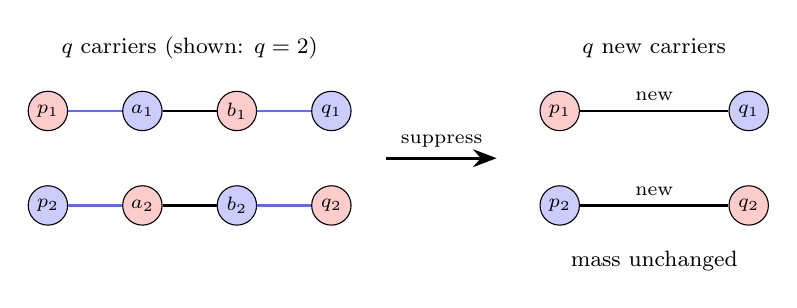
\begin{tikzpicture}[
  vertex/.style={circle, draw, minimum size=5mm, inner sep=0pt, font=\scriptsize},
  rv/.style={vertex, fill=red!20},
  bv/.style={vertex, fill=blue!20},
  >=Stealth
]
\begin{scope}[local bounding box=parent]
  \node[rv] (p1) at (0,1.2) {$p_1$};
  \node[bv] (a1) at (1.2,1.2) {$a_1$};
  \node[rv] (b1) at (2.4,1.2) {$b_1$};
  \node[bv] (q1) at (3.6,1.2) {$q_1$};
  \draw[thick] (a1) -- (b1);
  \draw[thick,blue!60] (p1) -- (a1);
  \draw[thick,blue!60] (b1) -- (q1);

  \node[bv] (p2) at (0,0) {$p_2$};
  \node[rv] (a2) at (1.2,0) {$a_2$};
  \node[bv] (b2) at (2.4,0) {$b_2$};
  \node[rv] (q2) at (3.6,0) {$q_2$};
  \draw[thick] (a2) -- (b2);
  \draw[thick,blue!60] (p2) -- (a2);
  \draw[thick,blue!60] (b2) -- (q2);

  \node[font=\footnotesize] at (1.8,2) {$q$ carriers (shown: $q=2$)};
\end{scope}

\draw[-{Stealth[length=3mm]}, very thick] (4.3, 0.6) --
  node[above, font=\scriptsize] {suppress} (5.7, 0.6);

\begin{scope}[xshift=6.5cm]
  \node[rv] (p1') at (0,1.2) {$p_1$};
  \node[bv] (q1') at (2.4,1.2) {$q_1$};
  \draw[thick] (p1') -- node[above,font=\scriptsize] {new} (q1');

  \node[bv] (p2') at (0,0) {$p_2$};
  \node[rv] (q2') at (2.4,0) {$q_2$};
  \draw[thick] (p2') -- node[above,font=\scriptsize] {new} (q2');

  \node[font=\footnotesize] at (1.2,2) {$q$ new carriers};
  \node[font=\footnotesize] at (1.2,-.7) {mass unchanged};
\end{scope}
\end{tikzpicture}
\caption{The multi-carrier funnel step with $q = 2$ carriers.  Each
bichromatic carrier $a_ib_i$ is extended to a switch block, the internal
vertices are suppressed, and the new bichromatic carrier $p_iq_i$
replaces it.  The background restriction mass is invariant.}
\label{fig:multi-carrier-funnel}
\end{figure}

\begin{lemma}[Multi-carrier pattern isolation]
\label{lem:multi-carrier-isolation}
No monochromatic $1$-rectangle in $M(I, S_\chi)$ can contain $1$-entries
from two local-state patterns $\eta \neq \eta'$.
\end{lemma}

\begin{proof}
$\eta$ and $\eta'$ differ on some block $W_i$.  Since $W_i$ is
degree-visible, the mixed graph $L_{S_\chi}(H_1) \cup R_{S_\chi}(H_0)$
has a vertex of degree $\neq 2$ and is non-Hamiltonian
(Theorem~\ref{thm:open-switch-anti-sharing}).
\end{proof}

\subsubsection*{The multi-carrier funnel recurrence}

\begin{theorem}[One-step multi-carrier magnification]
\label{thm:multi-carrier-magnification}
For all sufficiently large $N$,
\[
\Gamma_q(N) \;\ge\; 2^q\,\Gamma_q(N - 2q).
\]
\end{theorem}

\begin{proof}
Choose $(I^\star, \chi^\star, \mathcal{E}^\star) \in \mathcal{C}_{N,q}$
attaining $\Gamma_q(N)$.  By
Lemma~\ref{lem:multi-carrier-extension-existence}, obtain a multi-carrier
extension with $q$ blocks $W_1, \ldots, W_q$.

By Lemma~\ref{lem:multi-carrier-isolation}, no monochromatic $1$-rectangle
meets two distinct pattern blocks.  By restriction monotonicity,
\[
\mathrm{pp}_1(I^\star, S_{\chi^\star})
\;\ge\; \sum_{\eta \in \{0,1\}^q} \mathrm{pp}_1(Q_\eta).
\]

By Lemma~\ref{lem:multi-carrier-suppression}, each pattern block
$Q_\eta \cong M(I_\eta, S_{\chi^\star,\eta})$ for a
multi-carrier-admissible child of size $N - 2q$.  Hence
$\mathrm{pp}_1(Q_\eta) \ge \Gamma_q(N - 2q)$.

So $\Gamma_q(N) \ge 2^q \cdot \Gamma_q(N - 2q)$.
\end{proof}

\begin{corollary}[Iterated multi-carrier recurrence]
\label{cor:multi-carrier-recurrence}
$\Gamma_q(N) \ge 2^{\Omega(N)}$ for $q = (\log N)^A$ and all
sufficiently large $N$.
\end{corollary}

\begin{proof}
Choose a fixed base size $N_0 = C_0 q^2$ for a sufficiently large
constant $C_0$.  Then $\Gamma_q(N_0) \ge 1$: a multi-carrier-admissible
instance of size $N_0$ carries a restriction of size
$|\rho| = O(q) = O(\sqrt{N_0})$, which is $o(N_0)$, so
Theorem~\ref{thm:packed-family} (restriction robustness) gives
$|\mathcal{P}_{N_0}[\rho]| = 2^{\Theta(N_0 \log N_0)} \ge 1$ for
$N_0$ large enough, yielding $\mathrm{pp}_1 \ge 1$.
Iterate Theorem~\ref{thm:multi-carrier-magnification} for
$\lfloor(N - N_0)/(2q)\rfloor$ steps:
\[
\Gamma_q(N) \ge 2^{q \cdot \lfloor(N-N_0)/(2q)\rfloor} \cdot \Gamma_q(N_0)
= 2^{\Omega(N)}.  \qedhere
\]
\end{proof}

\subsection{The Formula Lower Bound via Protocol-Partition Numbers}

\begin{definition}[One-sided protocol-partition number]
\label{def:pp1}
For a Boolean function $f$ and variable partition $S$, $\mathrm{pp}_1(f,S)$
is the minimum number of $1$-leaves in any protocol-partition tree for $M(f,S)$.
For a restricted instance $I = \mathcal{P}_n[\rho]$, write
$\mathrm{pp}_1(I, S) := \mathrm{pp}_1(f_I, S)$ where $f_I$ is the
characteristic function of $I$.
\end{definition}

\begin{proposition}[Aho--Ullman--Yannakakis {\cite{AUY83}}]
\label{prop:auy}
If $F$ is a formula of size $L$ computing $f$, then
$\mathrm{pp}_1(f, S) \le L$ for every partition $S$.
\end{proposition}

\begin{lemma}[Cross-pattern rectangle isolation]
\label{lem:rect-isolation}
No monochromatic $1$-rectangle in $M(I, S)$ can contain $1$-entries from
two distinct pattern blocks $Q_\eta, Q_{\eta'}$ with $\eta \neq \eta'$.
\end{lemma}

\begin{proof}
A $1$-rectangle containing entries from both $Q_\eta$ and $Q_{\eta'}$
would force acceptance of the mixed input $(x_L^{\eta'}, x_R^\eta)$.
By Theorem~\ref{thm:open-switch-anti-sharing}, this mixed graph is
non-Hamiltonian.  Contradiction.
\end{proof}

\begin{definition}[Recursive measure]
\label{def:lambda}
$\Lambda(n) := \Gamma_q(n)$ from Definition~\ref{def:multi-carrier-admissible},
with $q = (\log n)^A$.
\end{definition}

\begin{corollary}[Formula lower bound]
\label{cor:formula-lower-bound}
Every Boolean formula computing $\Ham_n$ has size $\ge 2^{\Omega(n)}$.
\end{corollary}

\begin{proof}
Fix a balanced coloring $\chi : [n] \to \{R, B\}$ and let $S_\chi$ be
its chromatic frontier.  By the Aho--Ullman--Yannakakis characterization
(Proposition~\ref{prop:auy}), $\mathrm{pp}_1(\Ham_n, S_\chi) \le |F|$
for any formula $F$ computing $\Ham_n$.

\textbf{Seed step.}
By Theorem~\ref{thm:disjoint-switch-packing} (with the doubly bichromatic
variant) applied to the unrestricted instance under coloring $\chi$, pack
$q = (\log n)^A$ disjoint, open, degree-visible switch blocks
$W_1, \ldots, W_q$ with $\chi(a_i) \neq \chi(b_i)$ and
$\chi(p_i) \neq \chi(q_i)$ for every $i$.
By Lemma~\ref{lem:rect-isolation}, the $2^q$ pattern blocks are isolated.
Suppressing the internal vertices of all blocks creates $q$ port edges,
which serve as the initial carriers.  The child instances are
multi-carrier-admissible of size $n - 2q$ with restriction $O(q) =
(\log n)^{O(1)}$.

\textbf{Funnel iteration.}
By Corollary~\ref{cor:multi-carrier-recurrence},
$\Gamma_q(n - 2q) \ge 2^{\Omega(n)}$.

\textbf{Combining.}
\[
|F| \;\ge\; \mathrm{pp}_1(\Ham_n, S_\chi)
\;\ge\; 2^q \cdot \Gamma_q(n - 2q)
\;\ge\; 2^{\Omega(n)}.  \qedhere
\]
\end{proof}

\subsection{Width-to-Size for General Circuits via a Legal Monotone Lift}
\label{subsec:width-to-size}

For circuits with sharing, the protocol-partition recurrence does not
directly apply because a single physical gate may be reused across many
recursion branches.  The only additional issue for arbitrary Boolean
circuits is negation.  We remove that issue by passing to a monotone lift
on a legal doubled-variable slice.

For each edge variable $x_e$ of the original Hamiltonian-Cycle input,
introduce two positive variables $x_e^+$ and $x_e^-$, intended to encode
presence and absence of the edge.  A \emph{legal encoding} of a graph
$G\subseteq\binom{[n]}{2}$ is the point $\mathrm{enc}(G)$ defined by
\[
\mathrm{enc}(G)(x_e^+)=\mathbf{1}[e\in G],
\qquad
\mathrm{enc}(G)(x_e^-)=\mathbf{1}[e\notin G].
\]
Thus every legal input satisfies $x_e^++x_e^-=1$ for every edge $e$.

We replace an arbitrary Boolean circuit by a monotone fan-in-$2$ circuit
on the variables $\{x_e^+,x_e^-:e\in\binom{[n]}{2}\}$ that agrees with
the original circuit on the legal slice.  The separator-interface
geometry, switch blocks, pattern blocks, and mixed-input constructions
are then read on legal encodings, with both literals of each edge placed
on the same side of every frontier.  On that legal slice, left/right
mixing in the lifted variable space is exactly the original edge mixing.
Hence the entire Hamiltonian anti-stitch framework applies verbatim.

\begin{proposition}[Linear legal monotone lift]
\label{prop:legal-monotone-lift}
Let $C$ be any fan-in-$2$ Boolean circuit of size $s$ computing a
function of the edge variables $\{x_e:e\in\binom{[n]}{2}\}$.  Then there
exists a monotone fan-in-$2$ circuit $C^{\pm}$ on the doubled variables
$\{x_e^+,x_e^-:e\in\binom{[n]}{2}\}$ with size at most $2s$ such that
for every graph $G\subseteq\binom{[n]}{2}$,
\[
C^{\pm}(\mathrm{enc}(G))=C(G).
\]
More generally, for every gate $g$ of $C$ there are monotone gates
$g^+,g^-$ in $C^{\pm}$ such that for every legal encoding
$\mathrm{enc}(G)$,
\[
g^+(\mathrm{enc}(G))=g(G),
\qquad
g^-(\mathrm{enc}(G))=1-g(G).
\]
\end{proposition}

\begin{proof}
Process the gates of $C$ in topological order.

If $g$ is an input variable $x_e$, define $g^+:=x_e^+$ and $g^-:=x_e^-$.
On every legal encoding, $x_e^+=1$ iff $e\in G$ and $x_e^-=1$ iff
$e\notin G$, so the claim holds.

If $g=\neg h$, define $g^+:=h^-$ and $g^-:=h^+$.  No new monotone gate
is needed.

If $g=h_1\vee h_2$, define $g^+:=h_1^+\vee h_2^+$ and
$g^-:=h_1^-\wedge h_2^-$.

If $g=h_1\wedge h_2$, define $g^+:=h_1^+\wedge h_2^+$ and
$g^-:=h_1^-\vee h_2^-$.

An induction on the topological order shows that on every legal encoding,
$g^+$ computes the value of $g$ and $g^-$ computes its complement.
The output of $C^{\pm}$ is $o^+$, where $o$ is the output gate of $C$.
Every original $\wedge/\vee$ gate contributes exactly two monotone gates,
while $\neg$ contributes none, so $|C^{\pm}|\le 2s$.
\end{proof}

\begin{proposition}[Frontier compatibility on the legal slice]
\label{prop:legal-frontier-compatibility}
Let $S$ be a frontier in the original edge-variable ordering, and let
$S^{\pm}$ be the lifted frontier obtained by placing both variables
$x_e^+,x_e^-$ on the same side of the frontier as the original edge
variable $x_e$.

Then for any two Hamiltonian cycles $H,H'$,
\[
\bigl(\mathrm{enc}(H')_{L^{\pm}},\;\mathrm{enc}(H)_{R^{\pm}}\bigr)
=\mathrm{enc}\bigl(L_S(H')\cup R_S(H)\bigr).
\]
In particular:
\begin{enumerate}
\item legal inputs are closed under left/right mixing;
\item balanced frontiers remain balanced after lifting;
\item every separator-interface state, switch-block pattern, and
  cross-pattern mixed graph from the original framework is realized
  identically on the legal slice of the lifted variable space.
\end{enumerate}
\end{proposition}

\begin{proof}
Fix an edge $e$.  If $e\in E_{\le S}$, then in the mixed point both
literals $x_e^+,x_e^-$ are taken from $\mathrm{enc}(H')$, hence
$x_e^+=\mathbf{1}[e\in H']$ and $x_e^-=\mathbf{1}[e\notin H']$.
Thus the mixed point records exactly whether $e$ belongs to the left
partial graph $L_S(H')$.

If $e\in E_{>S}$, both literals are taken from $\mathrm{enc}(H)$, hence
$x_e^+=\mathbf{1}[e\in H]$ and $x_e^-=\mathbf{1}[e\notin H]$.
Thus the mixed point records exactly whether $e$ belongs to the right
partial graph $R_S(H)$.

Therefore, edge by edge, the mixed lifted assignment is precisely the
legal encoding of the mixed graph $L_S(H')\cup R_S(H)$.  Closure of
legality is immediate because each pair $(x_e^+,x_e^-)$ still sums
to~$1$.  Since the lift duplicates every original edge variable on the
same side of the frontier, all left/right counts are doubled uniformly,
so balance is preserved.  The separator-interface and switch-block
constructions depend only on the underlying mixed edge set, which is
unchanged.
\end{proof}

\begin{definition}[Branch history and gate-sharing multiplicity]
\label{def:gate-sharing-multiplicity}
For a valid magnification tree $R$ built by the multi-carrier funnel
and the lifted monotone circuit $C^{\pm}$, each internal node $\nu$
carries $q$ carrier extension blocks (with $q = (\log n)^A$ constant
across levels), hence $2^q$ child patterns.  For a descendant $\beta$, let
\[
\mathrm{Hist}(\beta) := (\eta_\nu(\beta))_{\nu \prec \beta},
\qquad \eta_\nu(\beta) \in \{0,1\}^{q_\nu},
\]
be its full ancestor pattern history.

For each leaf $\beta$ of $R$, let $G_\beta$ be the set of gates of
$C^\pm$ that appear in the protocol-partition tree induced by $C^\pm$
at the admissible pair $(I_\beta, S_\beta)$; equivalently, $G_\beta$
is the set of gates $g$ such that the subtree of $C^\pm$ rooted at $g$
contributes a $1$-leaf to the protocol-partition tree at $\beta$.

For a gate $g$ of $C^{\pm}$, define
\[
\mathcal{H}_g(R) := \{\mathrm{Hist}(\beta) : \beta \text{ is a leaf of }
R,\; g \in G_\beta\}.
\]
The \emph{multiplicity} of $g$ is $\mu(g) := |\mathcal{H}_g(R)|$, and
$\mu_{\max}(R,C^{\pm}) := \max_g \mu(g)$.
\end{definition}

\begin{proposition}[Width budget with sharing]
\label{prop:width-budget-sharing}
$\sum_\alpha w_\alpha \le K\,|C^{\pm}|\,\mu_{\max}(R,C^{\pm})$.
\end{proposition}

\begin{proof}
For each leaf $\alpha$ of $R$, the protocol-partition tree $T_\alpha$
for $(I_\alpha, S_\alpha)$ is built from $C^{\pm}$ via the standard
Karchmer--Wigderson construction: at each internal node, Alice and Bob
follow the evaluation of $C^{\pm}$ on their respective inputs, and the
protocol branches according to which child of the current gate is
explored.  Each $1$-leaf $\ell$ of $T_\alpha$ corresponds to a unique
accepting evaluation path $\pi(\ell)$ through $C^{\pm}$ --- the
sequence of gates visited from the output gate down to a $1$-input ---
and a monochromatic $1$-rectangle.

Define the gate-charging map $\kappa_\alpha$ by sending each $1$-leaf
$\ell$ to the \emph{branching gate} of $\pi(\ell)$: the deepest gate $g$
on $\pi(\ell)$ at which $\pi(\ell)$ diverges from the path of at least
one other $1$-leaf.  If $\ell$ is the unique $1$-leaf, charge it to the
output gate.  More precisely, for an OR gate $g$ on $\pi(\ell)$ with
children $g_0, g_1$, the protocol sends $\ell$ to child $g_{\ell}$; if
any other $1$-leaf $\ell'$ is sent to the opposite child $g_{1-\ell}$
at this node, then $g$ is a branching point of $\pi(\ell)$.  Set
$\kappa_\alpha(\ell)$ to be the topologically deepest such branching
gate (with ties broken by topological index).

The map $\kappa_\alpha$ is injective.  Suppose $\ell_1 \neq \ell_2$
are distinct $1$-leaves with $\kappa_\alpha(\ell_1)
= \kappa_\alpha(\ell_2) = g$.  Since $\ell_1$ and $\ell_2$ are
distinct leaves of the protocol tree, their evaluation paths must
diverge at some gate $g'$.  At $g'$, the two paths go to different
children; this makes $g'$ a branching point for both $\ell_1$ and
$\ell_2$.  If $g'$ is deeper than $g$, then $g$ is not the deepest
branching point of $\pi(\ell_1)$, contradicting the definition of
$\kappa_\alpha$.  If $g'$ is shallower or equal to $g$, then $\ell_1$
and $\ell_2$ diverge at $g'$ and follow disjoint subtrees below $g'$;
but both were charged to $g$, which is at depth $\ge g'$, so $g$ lies
in only one of the two subtrees below $g'$.  The leaf in the other
subtree cannot have $g$ on its path, contradicting
$\kappa_\alpha(\ell_2) = g$.  In either case we reach a contradiction,
so $\kappa_\alpha$ is injective.

Hence $w_\alpha = |L_1(T_\alpha)| \le |\mathrm{im}(\kappa_\alpha)|
\le |G_\alpha|$, where $G_\alpha$ is the set of physical gates charged
at $\alpha$.

Now double-count over (gate, leaf) pairs.  A physical gate $g$ belongs to
$G_\alpha$ only if $g$ has at least one occurrence in the canonical
accepting proof tree $T(z_\alpha)$ and that occurrence certifies a
$1$-rectangle on $(I_\alpha, S_\alpha)$.  The number of leaves $\alpha$
with $g \in G_\alpha$ is at most $\mu(g)$ (the number of distinct branch
histories at which $g$ is active, per
Definition~\ref{def:gate-sharing-multiplicity}).  Therefore
\[
\sum_\alpha w_\alpha
\;\le\; \sum_\alpha |G_\alpha|
\;=\; \sum_g |\{\alpha : g \in G_\alpha\}|
\;\le\; \sum_g \mu(g)
\;\le\; |C^{\pm}| \cdot \mu_{\max}.
\]
The constant $K$ absorbs the $O(1)$ protocol overhead per gate.
\end{proof}

\begin{proposition}[Leaf-sum domination of the root protocol-partition number]
\label{prop:leaf-sum-domination}
Fix a valid magnification tree $R$ rooted at an admissible pair $(I, S)$. For each leaf $\alpha$ of
$R$, let $(I_\alpha, S_\alpha)$ be the admissible pair carried by $\alpha$, and write
\[
w_\alpha := pp_1(I_\alpha, S_\alpha).
\]
Then
\[
pp_1(I, S) = \sum_{\alpha \text{ leaf of } R} w_\alpha.
\]
In particular, if $(I, S)$ realizes $\Lambda(n)$, then $\Lambda(n) = \sum_\alpha w_\alpha$.
\end{proposition}

\begin{proof}
We prove equality by induction on the depth of the valid magnification
tree.

If $R$ has depth $0$, then the root is itself a leaf, so the claim is
tautological.

Assume now that the root $\nu$ is an internal node carrying $q_\nu$
disjoint open switch blocks, with pattern blocks
\[
Q_{\nu,\eta} \subseteq M(I, S),\qquad \eta \in \{0,1\}^{q_\nu}.
\]
By construction of the magnification step, the accepted $1$-inputs of
$M(I, S)$ decompose across these pattern blocks, and by cross-pattern
rectangle isolation
(Lemma~\ref{lem:rect-isolation}) no monochromatic
$1$-rectangle can contain $1$-entries from two distinct pattern blocks.

\emph{Lower bound ($\ge$).}
Any protocol-partition tree computing $M(I, S)$ must decompose its
$1$-leaves as a disjoint union of $1$-leaves assigned separately to the
matrices induced on each pattern block $Q_{\nu,\eta}$.  Each child block
requires at least $pp_1(I_\eta, S_\eta)$ such $1$-leaves.  Therefore
\[
pp_1(I, S) \ge \sum_{\eta \in \{0,1\}^{q_\nu}} pp_1(I_\eta, S_\eta).
\]

\emph{Upper bound ($\le$).}
Conversely, take an optimal protocol-partition tree for each child
$(I_\eta, S_\eta)$, using exactly $pp_1(I_\eta, S_\eta)$ many
$1$-leaves.  Since the pattern blocks partition the $1$-entries of
$M(I, S)$, concatenating these child trees (with a single branching node
at the root that queries the switch-block pattern $\eta$) yields a valid
protocol-partition tree for $(I, S)$ with exactly
$\sum_\eta pp_1(I_\eta, S_\eta)$ many $1$-leaves.  Therefore
\[
pp_1(I, S) \le \sum_{\eta \in \{0,1\}^{q_\nu}} pp_1(I_\eta, S_\eta).
\]

Combining gives equality at one magnification step.  By induction, for
each child $\eta$,
$pp_1(I_\eta, S_\eta) = \sum_{\alpha \text{ leaf below } \eta} w_\alpha$.
Summing over all children gives
\[
pp_1(I, S) = \sum_{\alpha \text{ leaf of } R} w_\alpha. \qedhere
\]
\end{proof}


\begin{definition}[Canonical accepting proof tree on the legal monotone lift]
\label{def:canonical-proof-tree}
Fix a Boolean fan-in-$2$ circuit $C$ computing $\Ham_n$, and let
$C^{\pm}$ be its legal monotone lift from
Proposition~\ref{prop:legal-monotone-lift}.

For every legal accepted input $z=\mathrm{enc}(H)$, define the canonical
accepting proof tree $T(z)$ inside $C^{\pm}$ by: at each OR gate choose
the lexicographically first child evaluating to $1$ on $z$, and at each
AND gate keep both children.
\end{definition}

\begin{definition}[Mixed descendant slab at a node]
\label{def:mixed-descendant-slab}
Fix a valid magnification tree $R$, an internal node $\lambda$, and an
ancestor history $h$ above $\lambda$.

Let $\mathfrak{X}_{\lambda,h}$ be the set of accepted descendant witnesses
below $(\lambda,h)$, i.e.\ the legal encodings of Hamiltonian cycles whose
branch history agrees with $h$ above $\lambda$.

Define the \emph{mixed descendant slab}
\[
\mathfrak{S}_{\lambda,h}
:=\bigl\{\,M_\lambda(x_L,x_R):\,x_L,x_R\in\mathfrak{X}_{\lambda,h}\,\bigr\},
\]
where $M_\lambda(x_L,x_R)$ is the legal mixed input obtained by taking the
left side of $x_L$ and the right side of $x_R$ at the frontier of $\lambda$.

By Proposition~\ref{prop:legal-frontier-compatibility}, every point of
$\mathfrak{S}_{\lambda,h}$ is legal.  It need not be Hamiltonian.

Because the descendant switch blocks below $\lambda$ are pairwise
vertex-disjoint and their local flips commute, every point of
$\mathfrak{S}_{\lambda,h}$ is determined by a product choice of local
pair-states
\[
\sigma_{\xi,j}\in\Sigma:=\{00,01,10,11\}
\]
for each descendant switch block $W_{\xi,j}$ below $\lambda$: the first bit
records the state used by the left-source witness, the second the state used
by the right-source witness.

Thus $\mathfrak{S}_{\lambda,h}$ is a finite product family over the alphabet
$\Sigma$, on a common fixed background outside the descendant switch gadgets.
\end{definition}

\begin{definition}[$\Sigma$-sticky family]
\label{def:sigma-sticky-family}
Let $A$ be a finite alphabet and let $M\subseteq A^q$.  For
$J\subseteq[q]$, say $M$ is \emph{$J$-sticky} if there exists a background
word $\zeta\in A^{[q]\setminus J}$ such that
$\eta|_{[q]\setminus J}=\zeta$ for every $\eta\in M$.

For the mixed slabs above, the relevant alphabet is
$A=\Sigma=\{00,01,10,11\}$.
\end{definition}

\begin{definition}[Canonical continuation packet]
\label{def:continuation-packet}
Fix a legal accepted input $z$, and let $T(z)$ be the canonical accepting
proof tree in the lifted monotone circuit $C^{\pm}$
(Definition~\ref{def:canonical-proof-tree}).

Let $u$ be an occurrence-node of $T(z)$, and let
\[
a_0\to a_1\to\cdots\to a_m=u
\]
be the root-to-$u$ path in $T(z)$.

For each AND ancestor $a_j$ on that path, let $b_j$ be the sibling child
not on the path to $u$.

The \emph{continuation packet} $\Pi_z(u)$ is the rooted monotone formula
obtained by:
\begin{enumerate}
\item keeping the root-to-$u$ path $a_0,\dots,a_m$,
\item keeping every AND-sibling root $b_j$ as a leaf-placeholder,
\item replacing the entire subtree below $u$ by a leaf-placeholder
  labeled~$u$.
\end{enumerate}

For any legal input $x$, $\Pi_z(u)(x)$ is the value of that formula when
each placeholder is evaluated by the corresponding gate value in $C^{\pm}$
on $x$.
\end{definition}

\begin{lemma}[Packet acceptance]
\label{lem:packet-acceptance}
For every legal input $x$,
\[
\Pi_z(u)(x)=1\;\Longrightarrow\;C^{\pm}(x)=1.
\]
\end{lemma}

\begin{proof}
The root of $\Pi_z(u)$ is the output gate of $C^{\pm}$.  Every OR node on
the packet keeps exactly the branch used in $T(z)$, and every AND node
keeps both the path-child and the sibling placeholder.  If all packet
leaves evaluate to $1$ on $x$, then by upward induction every internal
node of the packet evaluates to $1$, hence the output gate of $C^{\pm}$
evaluates to $1$.
\end{proof}

\begin{definition}[Packet trace on a mixed slab]
\label{def:packet-trace-mixed-slab}
Fix $(\lambda,h)$, an accepted witness $z\in\mathfrak{X}_{\lambda,h}$, and
an occurrence $u\in T(z)$.

The \emph{packet trace} of $u$ on the mixed slab $\mathfrak{S}_{\lambda,h}$
is
\[
\Theta_{\lambda,h,z,u}
:=\Pi_z(u)\big|_{\mathfrak{S}_{\lambda,h}}.
\]

At an internal descendant node $\xi\succeq\lambda$ with $q_\xi$ switch
blocks, define the \emph{mixed child set}
\[
C_{\xi,h_\xi}^{\mathrm{mix}}(\Pi_z(u))\subseteq\Sigma^{q_\xi}
\]
to be the set of local pair-patterns $\eta$ for which the packet trace on
the corresponding child mixed slab is not identically zero.

Define the \emph{mixed free-coordinate set}
\[
F_{\xi,h_\xi}^{\mathrm{mix}}(\Pi_z(u))
:=\min\bigl\{J\subseteq[q_\xi]:
C_{\xi,h_\xi}^{\mathrm{mix}}(\Pi_z(u))\text{ is }J\text{-sticky}\bigr\}.
\]
\end{definition}

\begin{lemma}[Mixed local clog]
\label{lem:mixed-local-clog}
For every $\xi$, $h_\xi$, $z$, $u$:
\[
\bigl|C_{\xi,h_\xi}^{\mathrm{mix}}(\Pi_z(u))\bigr|
\le 4^{\,|F_{\xi,h_\xi}^{\mathrm{mix}}(\Pi_z(u))|}.
\]
\end{lemma}

\begin{proof}
Outside the minimal sticky set
$F_{\xi,h_\xi}^{\mathrm{mix}}(\Pi_z(u))$, every element of the mixed child
set has the same symbol in $\Sigma$.  Hence the mixed child set is contained
in a $|F^{\mathrm{mix}}|$-dimensional subcube of $\Sigma^{q_\xi}$, and each
free coordinate has at most $4$ possible symbols.
\end{proof}

\begin{theorem}[Branching-product multiplicity bound via mixed packets]
\label{thm:branching-product-mixed}
For a fixed physical gate $g$, and for each leaf $\beta$ with
$g\in G_\beta$, choose the first occurrence of $g$ in the canonical proof
tree $T(z_\beta)$ under a fixed preorder.  Let $\Pi_\beta(g)$ be its
continuation packet.

Then the number of distinct branch histories at which $g$ appears satisfies
\[
\mu(g)
\le\prod_{k=1}^{D}\max_{h}\,
\bigl|C_{\nu_k,h}^{\mathrm{mix}}(\Pi(g))\bigr|
\le 4^{\,\tau_{\mathrm{mix}}^*(g)},
\]
where
\[
\tau_{\mathrm{mix}}^*(g)
:=\sum_{k=1}^{D}\max_{h}\,
\bigl|F_{\nu_k,h}^{\mathrm{mix}}(\Pi(g))\bigr|.
\]
\end{theorem}

\begin{proof}
A branch history for an appearance of $g$ determines, level by level, a
diagonal local pair-state in each mixed child set for the distinguished
continuation packet of that appearance.  At each internal node $\nu_k$,
the number of surviving child choices is bounded by the corresponding
mixed child set size.  Multiply level by level and apply
Lemma~\ref{lem:mixed-local-clog}.
\end{proof}

\begin{lemma}[Mixed-slab corridor locality]
\label{lem:mixed-slab-corridor-locality}
Fix $(\lambda,h)$, an accepted witness $z\in\mathfrak{X}_{\lambda,h}$, an
occurrence $u\in T(z)$, and a corridor
$D\subseteq V(H_\lambda^\star)$.

For each descendant internal node $\xi\succeq\lambda$, let $D_\xi$ be the
descendant image of $D$.

Assume that for every active descendant level $\xi$ below $\lambda$,
\[
F_{\xi,h_\xi}^{\mathrm{mix}}(\Pi_z(u))
\]
is supported only on switch blocks contained in $D_\xi$.

Then there exists a Boolean function $\Psi_{\lambda,h,z,u,D}$ on the legal
variables with both endpoints in the descendant image $D_\beta$ such that
for every mixed input $x\in\mathfrak{S}_{\lambda,h}$,
\[
\Pi_z(u)(x)=\Psi_{\lambda,h,z,u,D}(x|_{D_\beta}).
\]
\end{lemma}

\begin{proof}
On the mixed slab $\mathfrak{S}_{\lambda,h}$, every descendant switch block
contributes a local pair-state in $\Sigma$, and the background outside
descendant switch gadgets is fixed.

If a switch block $W_{\xi,j}$ lies outside $D_\xi$, then by hypothesis
$j\notin F_{\xi,h_\xi}^{\mathrm{mix}}(\Pi_z(u))$.
So the mixed child set is sticky in coordinate $j$: every
packet-surviving local pair-pattern has the same $\Sigma$-symbol there.
Hence that local pair-state is frozen across the entire
packet-supporting slab.

Iterating from $\lambda$ down the active descendant levels, every mixed
local pair-state outside the descendant corridor $D$ is frozen, while all
packet variation is confined to the descendant image $D_\beta$.  Since the
common background outside the descendant gadgets is fixed as well, the
value of the packet on $\mathfrak{S}_{\lambda,h}$ is a function only of the
legal variables inside $D_\beta$.
\end{proof}

\begin{corollary}[Mixed-slab packet persistence]
\label{cor:mixed-slab-packet-persistence}
In the setting of Lemma~\ref{lem:mixed-slab-corridor-locality}, let
$z\in\mathfrak{X}_{\lambda,h}$ and let
$M=M_\lambda(z',z)\in\mathfrak{S}_{\lambda,h}$ for some
$z'\in\mathfrak{X}_{\lambda,h}$.

Assume $M|_{D_\beta}=z|_{D_\beta}$ and $\Pi_z(u)(z)=1$.

Then $\Pi_z(u)(M)=1$, and therefore $C^{\pm}(M)=1$.
\end{corollary}

\begin{proof}
By Lemma~\ref{lem:mixed-slab-corridor-locality},
\[
\Pi_z(u)(M)
=\Psi_{\lambda,h,z,u,D}(M|_{D_\beta})
=\Psi_{\lambda,h,z,u,D}(z|_{D_\beta})
=\Pi_z(u)(z)=1.
\]
Now apply Lemma~\ref{lem:packet-acceptance}.
\end{proof}

This is the exact spot where the earlier gate-local argument failed: it
tried to conclude full acceptance from $g(M)=1$ for a single reused gate.
The repaired object is the whole continuation packet, so the AND-sibling
obligations are built into the localized object.  The mixed-slab domain
ensures that the non-Hamiltonian mixed input $M$ lies in the domain of the
packet-locality function $\Psi$, resolving the cube-versus-slab domain gap.

\begin{definition}[Marked corridor and descendant image]
\label{def:marked-corridor}
Let $\nu$ be an internal node of the magnification tree carrying $q$
switch blocks $W_{\nu,1}, \ldots, W_{\nu,q}$.  A \emph{marked corridor}
at level $\nu$ is a subset $D \subseteq V(H^\star_\nu)$ consisting of
the vertex support of one or more switch blocks: $D = \bigcup_{j \in J}
V(W_{\nu,j})$ for some $J \subseteq [q]$.

For each descendant level $\xi \succeq \nu$, the \emph{descendant image}
$D_\xi$ of $D$ is the image of $D$ under the composition of suppression
maps from $\nu$ to $\xi$.  Concretely, at each intermediate level the
suppression deletes the internal vertices of the suppressed blocks and
replaces through-paths by port edges; $D_\xi$ consists of the surviving
vertices of $D$ plus the port vertices that replaced carrier endpoints
belonging to $D$.  By the multi-carrier funnel's one-for-one carrier
replacement, the carrier lineages issued from $D$ remain well-defined
in $D_\xi$.
\end{definition}

\begin{definition}[First escape for a continuation packet]
\label{def:first-escape}
Fix an internal node $\nu$, an ancestor history $h$, a legal accepted
witness $z$ below $(\nu,h)$, a distinguished occurrence $u\in T(z)$, and
a marked corridor $D$ at level $\nu$
(Definition~\ref{def:marked-corridor}).

Assume that at level $\nu$ the packet has at least one mixed free
coordinate, and choose $D$ attached to one such
coordinate.

A \emph{first escape} of the packet from $D$ is a descendant active
level $\lambda\succeq\nu$ such that:
\begin{enumerate}
\item for every active level $\xi$ with $\nu\preceq\xi\prec\lambda$,
  every mixed free coordinate of the packet lies in the descendant
  image $D_\xi$; and
\item at level $\lambda$, there exists a mixed free coordinate
  $j_0\notin D_\lambda$.
\end{enumerate}

Fix such a first escape $\lambda$.  Choose an accepted descendant witness
$z'$ below $(\lambda,h_\lambda)$ such that:
\begin{itemize}
\item $z'$ agrees with $z$ on every descendant switch choice inside
  $D_\lambda$;
\item $z'$ and $z$ split for the first time at level $\lambda$, on the
  coordinate $j_0$.
\end{itemize}

Let $M:=M_\lambda(z',z)$.

We say that $j_0$ is
\begin{itemize}
\item \emph{packet-benign} if $\Pi_z(u)(M)=1$;
\item \emph{packet-separating} if $\Pi_z(u)(M)=0$.
\end{itemize}
\end{definition}

\begin{lemma}[Benign first escape is impossible]
\label{lem:benign-escape-impossible}
In the setting of Definition~\ref{def:first-escape}, a first escape
cannot be packet-benign.
\end{lemma}

\begin{proof}
Assume $\Pi_z(u)(M)=1$.  By Lemma~\ref{lem:packet-acceptance}, this
implies $C^{\pm}(M)=1$.

But $z$ and $z'$ agree above $\lambda$ and split for the first time at
$\lambda$, so $M$ is a cross-pattern mixed input at node $\lambda$.  By
Theorem~\ref{thm:open-switch-anti-sharing}, that mixed graph is
non-Hamiltonian; by Lemma~\ref{lem:rect-isolation}, such an input cannot
be accepted.  Contradiction.
\end{proof}

\begin{lemma}[Correct dichotomy at the first escape]
\label{lem:escape-dichotomy}
In the setting of Definition~\ref{def:first-escape}, if a first escape
exists at all, then it is necessarily packet-separating.
\end{lemma}

\begin{proof}
Immediate from Lemma~\ref{lem:benign-escape-impossible}.
\end{proof}

% -----------------------------------------------------------------------
% Rooted-packet descent package
% Closes the conditional gap in packet-separator exclusion (8.45--8.46).
% -----------------------------------------------------------------------

\begin{definition}[Rooted continuation packet]
\label{def:rooted-continuation-packet}
Fix a legal accepted input $z$ and an occurrence-node $r$ in the
canonical proof tree $T(z)$.  Let $u$ be a descendant occurrence of $r$
in $T(z)$, and write the root-to-$u$ path inside the rooted subtree
$T_r(z)$ as
\[
  r = a_0 \to a_1 \to \cdots \to a_m = u.
\]
For each AND ancestor $a_i$ on this rooted path, let $b_i$ be the
sibling child not on the path to $u$.

Define the \emph{rooted continuation packet} $\Pi^r_z(u)$ to be the
rooted monotone formula obtained by:
\begin{enumerate}
\item keeping the rooted path $a_0,\dots,a_m$,
\item keeping every rooted AND-sibling root $b_i$ as a leaf-placeholder,
\item replacing the entire subtree below $u$ by a leaf-placeholder
  labeled~$u$.
\end{enumerate}
For any legal input $x$, $\Pi^r_z(u)(x)$ is the value of that formula
when each placeholder is evaluated by the corresponding gate value in
$C^{\pm}$ on $x$.

When $r$ is the output gate of $C^{\pm}$, this coincides with the
ordinary continuation packet $\Pi_z(u)$.
\end{definition}

\begin{lemma}[Rooted packet acceptance]
\label{lem:rooted-packet-acceptance}
For every legal input $x$,
\[
  \Pi^r_z(u)(x) = 1 \;\Longrightarrow\; r(x) = 1.
\]
\end{lemma}

\begin{proof}
Upward induction inside the rooted packet.  Every OR node on the packet
keeps exactly the branch used in $T(z)$, and every AND node keeps both
the path-child and the sibling placeholder.  If all packet leaves
evaluate to $1$ on $x$, then by upward induction every internal node of
the packet evaluates to $1$, hence the root $r$ evaluates to $1$.
\end{proof}

\begin{lemma}[Rooted locality and rooted persistence]
\label{lem:rooted-locality-persistence}
Lemma~\ref{lem:mixed-slab-corridor-locality}
and Corollary~\ref{cor:mixed-slab-packet-persistence} remain valid verbatim for
rooted continuation packets, with the conclusion $r(M)=1$ in place of
$C^{\pm}(M)=1$.
\end{lemma}

\begin{proof}
The proofs of those lemmas use only packet structure on the mixed slab,
stickiness of mixed child sets, and upward evaluation inside the packet.
None of that depends on the packet root being the circuit output.
Replace the final appeal to Lemma~\ref{lem:packet-acceptance} by
Lemma~\ref{lem:rooted-packet-acceptance}.
\end{proof}

\begin{definition}[Uniform certification through level $\lambda$]
\label{def:uniform-certification}
Fix an internal node $\nu$, an ancestor history $h$, a legal accepted
witness $z$ below $(\nu,h)$, a rooted continuation packet
$P = \Pi^r_z(u)$, and a marked corridor $D \subseteq V(H^\star_\nu)$.

For any active descendant level $\xi \succeq \nu$, call an input
$N = M_\xi(w,z) \in \mathfrak{S}_{\xi,h_\xi}$ \emph{$D$-consistent at
level $\xi$} if the accepted descendant witness $w$ agrees with $z$ on
every descendant switch choice inside $D_\xi$.

Let $a$ be an AND-node on the unique occurrence-path in $T(z)$ from the
output gate of $C^\pm$ down to $u$.  Write $s(a)$ for the child of $a$
that does not lie on that path.

We say that $P$ is \emph{uniformly certified through level $\lambda$} if
for every such AND-node $a$, every active descendant level $\xi$ with
$\nu \preceq \xi \preceq \lambda$, and every $D$-consistent input $N$
at level $\xi$, one has $s(a)(N) = 1$.

Now let $\lambda$ be a first $D$-escape level for $P$, and let
$M := M_\lambda(z',z)$ be the mixed input attached to that first escape.
If $P$ is uniformly certified through level $\lambda$, the first escape
is a \emph{uniformly certified first $D$-escape}.

For a uniformly certified first $D$-escape:
\begin{itemize}
\item it is \emph{packet-benign} if $P(M) = 1$;
\item it is \emph{packet-separating} if $P(M) = 0$.
\end{itemize}
\end{definition}

\begin{lemma}[Uniform certified rooted acceptance]
\label{lem:uniform-certified-acceptance}
Fix the setting of Definition~\ref{def:uniform-certification}, and assume
that $P = \Pi^r_z(u)$ is uniformly certified through level $\lambda$.
Let $\xi$ be any active descendant level with $\nu \preceq \xi \preceq
\lambda$, and let $N = M_\xi(w,z)$ be any $D$-consistent input at level
$\xi$.  If $P(N) = 1$, then $C^\pm(N) = 1$.
\end{lemma}

\begin{proof}
By Lemma~\ref{lem:rooted-packet-acceptance}, $P(N) = 1$ implies
$r(N) = 1$.  Move upward from $r$ to the output gate along the unique
occurrence-path in $T(z)$.  If an ancestor $a$ on that path is an OR
gate, the child on the path already has value $1$, so $a(N) = 1$.  If
$a$ is an AND gate, the child on the path has value $1$, and the
off-path child is $s(a)$.  Since $P$ is uniformly certified through
$\lambda$ and $\xi \le \lambda$ and $N$ is $D$-consistent at level
$\xi$, we have $s(a)(N) = 1$.  Hence $a(N) = 1$.  Inducting upward,
$C^\pm(N) = 1$.
\end{proof}

\begin{lemma}[Uniform certified benign escape is impossible]
\label{lem:uniform-benign-impossible}
In the setting of Definition~\ref{def:uniform-certification}, a
uniformly certified first $D$-escape cannot be packet-benign.
\end{lemma}

\begin{proof}
Let $\lambda$ be the first $D$-escape level and $M := M_\lambda(z',z)$.
If $P(M) = 1$, Lemma~\ref{lem:uniform-certified-acceptance} yields
$C^\pm(M) = 1$.  But $M$ is a cross-pattern mixed input at level
$\lambda$, hence non-Hamiltonian.  Contradiction.
\end{proof}

\begin{lemma}[Initialization by globally highest failing gate]
\label{lem:initialization-highest-failing}
Suppose an ordinary continuation packet $\Pi_z(u)$ admits a
packet-separating first $D$-escape at level $\lambda$, witnessed by
$M = M_\lambda(z',z)$.

Then there exist: an occurrence-node $r$ in $T(z)$, an active descendant
level $\lambda_r$ with $\nu \preceq \lambda_r \preceq \lambda$, and a
$D$-consistent mixed input $N_r = M_{\lambda_r}(w_r, z)$, such that
for the trivial rooted packet $\Gamma_r := \Pi^r_z(r)$:
\begin{enumerate}
\item $\Gamma_r(z) = r(z) = 1$ and $\Gamma_r(N_r) = r(N_r) = 0$;
\item $\Gamma_r$ has a first $D$-escape at some active level
  $\tau_r \preceq \lambda_r$;
\item $\Gamma_r$ is uniformly certified through level $\tau_r$;
\item the first $D$-escape of $\Gamma_r$ at level $\tau_r$ is
  packet-separating.
\end{enumerate}
\end{lemma}

\begin{proof}
Because $M$ is a cross-pattern mixed input at level $\lambda$, it is
non-Hamiltonian, hence $C^\pm(M) = 0$.

Take $r$ to be the output gate of $C^{\pm}$, with $\lambda_r := \lambda$
and $N_r := M$.  Set $\Gamma_r := \Pi^r_z(r)$.  Then
$\Gamma_r(z) = C^{\pm}(z) = 1$ (since $z = \mathrm{enc}(H)$ is accepted)
and $\Gamma_r(N_r) = C^{\pm}(M) = 0$.

If $\Gamma_r$ had no first $D$-escape at any level $\xi \le \lambda$,
then all mixed free coordinates through level $\lambda$ would remain
inside the descendant image of $D$.  Since $M$ is $D$-consistent at
level $\lambda$, rooted persistence
(Lemma~\ref{lem:rooted-locality-persistence}) would imply
$\Gamma_r(M) = 1$, contradiction.  Hence $\Gamma_r$ has a first
$D$-escape at some level $\tau_r \preceq \lambda$.

$\Gamma_r$ is uniformly certified through level $\tau_r$: the
occurrence-path from the output gate to $r = \text{output gate}$ in
$T(z)$ is empty (a single node), so there are no AND-nodes on the path
and the certification condition is vacuously satisfied.

Finally, by Lemma~\ref{lem:uniform-benign-impossible}, the first
$D$-escape of $\Gamma_r$ at $\tau_r$ cannot be benign.  Hence it is
packet-separating.
\end{proof}

\begin{theorem}[Uniform certified rooted packet-separator exclusion]
\label{thm:packet-separator-exclusion}
Every packet-separating first $D$-escape of a uniformly certified
rooted continuation packet is a terminal single-variable escape at
rooted subtree height~$0$.

In particular, every packet-separating first escape of an ordinary
continuation packet is a terminal single-variable escape.
\end{theorem}

\begin{proof}
We prove the following by strong induction on rooted subtree height $h$:

\medskip
\noindent\textbf{Claim $\boldsymbol{I(h)}$.}
\emph{Let $P = \Pi^r_z(u)$ be a uniformly certified rooted continuation
packet at a root $r$ of rooted subtree height $\le h$, with a
packet-separating first $D$-escape at level $\lambda$ witnessed by
$M = M_\lambda(z',z)$.  Then $P$'s escape is a terminal single-variable
escape at rooted subtree height~$0$.}

\medskip

By Lemma~\ref{lem:uniform-benign-impossible}, a uniformly certified
first $D$-escape cannot be benign, so every first $D$-escape of a
certified packet is packet-separating.

\textbf{Base case ($h = 0$).}
The root $r$ is a leaf (input gate) and $u = r$.  The packet
$P = \Pi^r_z(r)$ computes a single lifted input variable $x_e^+$ or
$x_e^-$ for some edge $e$.

The edge $e$ belongs to at most one switch block $W_{\xi,j}$ at a single
active level $\xi$.  If $j \in D_\xi$, the packet has no free
coordinate outside $D$, hence no first $D$-escape.

If $j \notin D_\xi$, the packet has a first $D$-escape at level $\xi$.
This height-$0$ escape is a genuine single-variable separation.
We call it a \emph{terminal single-variable escape}: it occurs at
exactly one active level, contributes $|F^{\mathrm{mix}}| \le 1$ at
that level, and $0$ at all others.  This establishes $I(0)$.

\textbf{Inductive step ($h \ge 1$).}
Assume $I(h')$ for all $h' < h$.  Let $P = \Pi^r_z(u)$ at root $r$
of height $h$, uniformly certified through $\lambda$, with
$P(z) = 1$ and $P(M) = 0$.

Consider the trivial rooted packet $\Gamma_u := \Pi^u_z(u)$.
Since $\Gamma_u$ has root $u$ and distinguished occurrence $u$, the
occurrence-path from $u$ to $u$ is empty, so $\Gamma_u$ is vacuously
uniformly certified through level $\lambda$.

\emph{Case~A: $\Gamma_u$ has no first $D$-escape through level
$\lambda$.}
By rooted persistence
(Lemma~\ref{lem:rooted-locality-persistence}),
$u(M) = \Gamma_u(M) = 1$.
We show this case is vacuous.  By the first-escape definition
(Definition~\ref{def:first-escape}), $z'$ agrees with $z$ on every
switch choice inside $D_\lambda$, so $M$ is $D$-consistent at level
$\lambda$.  Since $P$ is uniformly certified through $\lambda$, every
AND-node $a_i$ on the occurrence-path from the output of $C^{\pm}$
to $u$ has its off-path sibling $b_i$ satisfying $b_i(M) = 1$.  In
particular, every AND-sibling on the $r$-to-$u$ portion of the path
evaluates to $1$ on $M$.  The rooted packet formula gives
$P(M) = u(M) \wedge \bigwedge_i b_i(M) = 1 \wedge 1 = 1$,
contradicting $P(M) = 0$.  So Case~A never arises.

\emph{Case~B: $\Gamma_u$ has a first $D$-escape at some level
$\xi \le \lambda$.}
By Lemma~\ref{lem:uniform-benign-impossible} (since $\Gamma_u$ is
certified), the escape is packet-separating.  Since
$\mathrm{ht}(u) < h$, by $I(\mathrm{ht}(u))$ the escape is a terminal
single-variable escape at height~$0$.  The gate $u$ fails on $M$
because of this terminal escape.  Since $u$ is on the accepting path
of $P$, $P$'s failure on $M$ traces through $u$ to the terminal
escape.  $I(h)$ holds.

\medskip

Since Case~A is vacuous, Case~B is the only possibility: every
packet-separating first $D$-escape of a uniformly certified rooted
packet at height $\le h$ is a terminal single-variable escape.
By induction, this holds for all~$h$.

For the ordinary continuation packet statement: if an ordinary
continuation packet admitted a packet-separating first $D$-escape,
Lemma~\ref{lem:initialization-highest-failing} would produce a uniformly
certified rooted continuation packet whose first $D$-escape is
packet-separating.  By the statement just proved, that escape
is a terminal single-variable escape.
\end{proof}

\begin{figure}[ht]
\centering
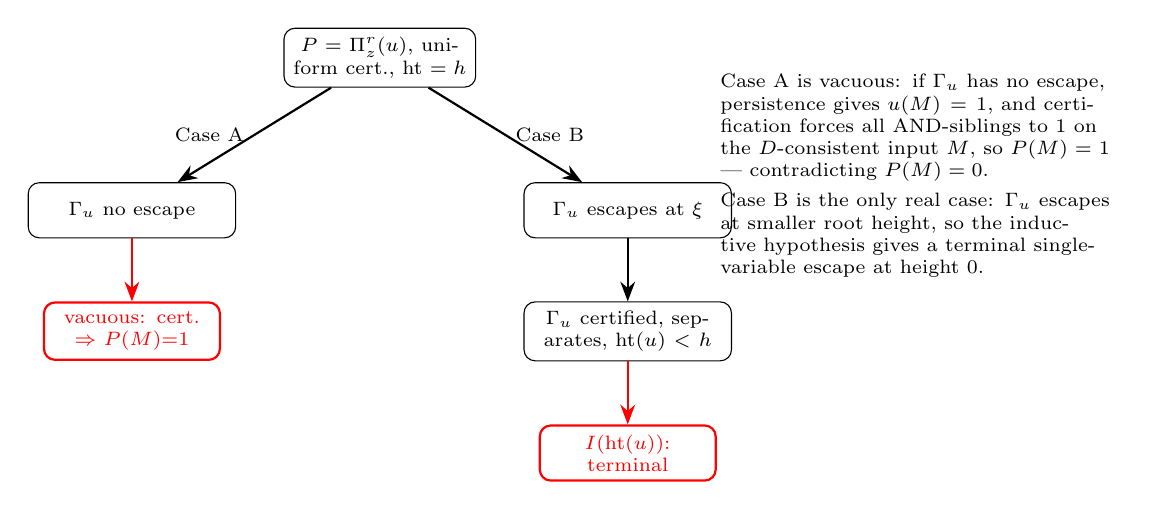
\begin{tikzpicture}[
  nd/.style={draw, rounded corners, minimum width=1.8cm, minimum height=0.7cm,
    font=\scriptsize, text centered},
  arr/.style={-{Stealth[length=2.5mm]}, thick},
  >=Stealth
]
\node[nd, text width=2.2cm] (r) at (0,0) {$P = \Pi^r_z(u)$, uniform cert., ht $= h$};
\node[nd, text width=2.4cm, below left=1.2cm and 0.6cm of r] (caseA)
  {$\Gamma_u$ no escape};
\node[nd, text width=2.4cm, below right=1.2cm and 0.6cm of r] (caseB)
  {$\Gamma_u$ escapes at $\xi$};

\draw[arr] (r) -- node[left, font=\scriptsize] {Case A} (caseA);
\draw[arr] (r) -- node[right, font=\scriptsize] {Case B} (caseB);

\node[draw=red, thick, rounded corners, below=0.8cm of caseA, font=\scriptsize,
  minimum width=2cm, text=red, text width=2cm, text centered] (vacuous)
  {vacuous: cert.\ $\Rightarrow$ $P(M){=}1$};
\draw[arr, red] (caseA) -- (vacuous);

\node[nd, text width=2.4cm, below=0.8cm of caseB] (ind)
  {$\Gamma_u$ certified, separates, ht$(u) < h$};
\draw[arr] (caseB) -- (ind);

\node[draw=red, thick, rounded corners, below=0.8cm of ind, font=\scriptsize,
  minimum width=2cm, text=red, text width=2cm, text centered] (term)
  {$I(\mathrm{ht}(u))$: terminal};
\draw[arr, red] (ind) -- (term);

\node[font=\scriptsize, text width=5cm, anchor=west] at (4.2, -1.5)
  {Case~A is vacuous: if $\Gamma_u$ has no
   escape, persistence gives $u(M)=1$,
   and certification forces all AND-siblings
   to~$1$ on the $D$-consistent input $M$,
   so $P(M)=1$ --- contradicting $P(M)=0$.\\[3pt]
   Case~B is the only real case: $\Gamma_u$
   escapes at smaller root height, so the
   inductive hypothesis gives a terminal
   single-variable escape at height~$0$.};
\end{tikzpicture}
\caption{Uniform-certified rooted descent
(Theorem~\ref{thm:packet-separator-exclusion}).  Case~A (no escape for
$\Gamma_u$) is vacuous: rooted persistence gives $u(M) = 1$, and
uniform certification forces every AND-sibling on the path to evaluate
to~$1$ on the $D$-consistent input~$M$, so $P(M) = 1$, contradicting
the hypothesis $P(M) = 0$.  The only real case is~B: $\Gamma_u$ has a
first $D$-escape at smaller root height, which by the inductive
hypothesis is a terminal single-variable escape at height~$0$.}
\label{fig:packet-descent}
\end{figure}

\begin{remark}[Terminal escape: complete logical chain]
\label{rem:terminal-escape-chain}
The treatment of height-$0$ terminal escapes is spread across three
locations; we collect the full logical chain here for the reader's
convenience.
\begin{enumerate}
\item \emph{Base case
(Theorem~\ref{thm:packet-separator-exclusion}, height $0$):}
A leaf gate $x_e$ whose edge $e$ belongs to a switch block outside the
corridor $D$ produces a genuine packet-separating first $D$-escape.
The rooted descent terminates at exactly one such leaf gate, yielding
\emph{at most one} terminal escape per descent chain, at a unique
active level $\xi_{\mathrm{term}}$ and coordinate
$j_{\mathrm{term}}$.
\item \emph{Recording
(Definition~\ref{def:occurrence-signature}, item 4):}
The occurrence signature records the terminal escape as a single triple
$(\xi_{\mathrm{term}}, j_{\mathrm{term}},
\mathrm{Hist}_{\xi_{\mathrm{term}}}(\beta)_{j_{\mathrm{term}}})$,
or is empty if no terminal escape occurs.
\item \emph{Closure
(Lemma~\ref{lem:signature-injectivity}, Step 5, Case $P(M) = 0$):}
If two leaves have the same signature and their histories differ at
level $\lambda$, the differing coordinate is neither in the lineage
set (signatures agree) nor the terminal escape (markers agree).
A non-terminal, non-lineage escape at height $\ge 1$ is excluded by
the inductive step.  A second terminal escape at height $0$ is
impossible (uniqueness from item 1).  Both cases yield a
contradiction, so the full history is determined by the signature.
\end{enumerate}
\end{remark}

\begin{definition}[Carrier lineage]
\label{def:carrier-lineage}
For a marked corridor $D$ at level $\nu$, let $L_\nu(D)$ be the set of
carrier indices whose switch blocks at level $\nu$ are contained in $D$.
For each later active descendant level $\xi \succeq \nu$, define
$L_\xi(D)$ inductively by following the unique descendant carrier spawned
from each carrier in $L_\nu(D)$.

Because each carrier is replaced by exactly one new carrier under the
multi-carrier funnel step, and different carriers remain pairwise
vertex-disjoint, the sets $L_\xi(D)$ are well-defined and satisfy
\[
|L_\xi(D)| = |L_\nu(D)|.
\]
When $D$ is chosen as the marked corridor containing one mixed free
coordinate, $D$ contains only $O(1)$ switch blocks initially; in the
minimal choice, $|L_\nu(D)| = 1$.
\end{definition}

\begin{lemma}[Carrier-lineage persistence bound]
\label{lem:carrier-lineage-persistence}
Fix an internal node $\nu$, an ancestor history $h$, a legal accepted
witness $z$ below $(\nu,h)$, and an occurrence $u \in T(z)$.  Suppose
the packet has a mixed free coordinate at level $\nu$.  Let $D$ be a
marked corridor containing one such coordinate, and let
$r := |L_\nu(D)|$.

Assume packet-separator exclusion, so that every later mixed free
coordinate of the packet along every consistent descendant branch lies
in the descendant image of $D$.  Then for every active descendant
level $\xi \succeq \nu$,
\[
F_{\xi,h_\xi}^{\mathrm{mix}}(\Pi_z(u)) \subseteq L_\xi(D),
\]
and therefore
$\bigl|F_{\xi,h_\xi}^{\mathrm{mix}}(\Pi_z(u))\bigr| \le r = O(1)$.
\end{lemma}

\begin{proof}
By packet-separator exclusion and the first-escape analysis, every later
mixed free coordinate lies in the descendant image $D_\xi$ of $D$.  The
only switch gadgets contained in $D_\xi$ are precisely the descendant
switch blocks belonging to the carrier lineages issued from the initial
carrier set $L_\nu(D)$: at each funnel step each old carrier is consumed
and replaced by exactly one new carrier, with no splitting, and different
carriers stay pairwise vertex-disjoint.  Hence $D_\xi$ contains exactly
the switch blocks indexed by $L_\xi(D)$, and
$|L_\xi(D)| = |L_\nu(D)| = r$.

If $j \notin L_\xi(D)$, then the switch block $W_{\xi,j}$ lies outside
$D_\xi$, so $j$ cannot be a mixed free coordinate.  Therefore
$F_{\xi,h_\xi}^{\mathrm{mix}}(\Pi_z(u)) \subseteq L_\xi(D)$.
Taking cardinalities gives the bound.
\end{proof}

% -----------------------------------------------------------------------
% Subexponential gate multiplicity via occurrence-signature rigidity.
%
% Strategy: rather than summing per-level mixed free-coordinate counts
% (which requires a union bound across levels), we define a compact
% per-leaf "occurrence signature" that records only the O(1) corridor-
% lineage coordinates at each active level.  The signature is injective
% on the set of leaves using a given gate (Lemma, via packet-separator
% exclusion + cross-pattern fatal mixing), and the codomain has size
% 2^{o(n)} (counting lemma).  This gives mu(g) <= 2^{o(n)} directly.
% -----------------------------------------------------------------------

\begin{definition}[Occurrence signature of a shared gate]
\label{def:occurrence-signature}
Fix a physical gate $g$ of $C^{\pm}$.  For each leaf $\beta$ of the
magnification tree $R$ with $g \in G_\beta$, let $u_\beta$ be the first
occurrence of $g$ in the canonical proof tree $T(z_\beta)$ under the
fixed preorder, and let
\[
P_\beta := \Pi_\beta(g) := \Pi_{z_\beta}(u_\beta)
\]
be the associated continuation packet.

If $P_\beta$ has no mixed free coordinate at any active level (i.e.\ the
packet is constant on the mixed slab at every level), define
$\mathrm{Sig}_g(\beta) := \bot$ (the \emph{null signature}).

Otherwise, let $\nu_\beta$ be the first active level at which $P_\beta$
has a mixed free coordinate.  Choose a marked corridor $D_\beta$ at level
$\nu_\beta$ containing one such coordinate.  For every active descendant
level $\xi \succeq \nu_\beta$, let
\[
L_\xi(\beta) := L_\xi(D_\beta)
\]
be the descendant carrier-lineage set issued from $D_\beta$
(Definition~\ref{def:carrier-lineage}).  By carrier-lineage persistence
and Lemma~\ref{lem:carrier-lineage-persistence},
$|L_\xi(\beta)| = r_\beta = O(1)$, and every mixed free coordinate of
$P_\beta$ at level $\xi$ lies in $L_\xi(\beta)$ (with the possible
exception of a unique terminal-escape coordinate).

Define the \emph{occurrence signature}
\[
\mathrm{Sig}_g(\beta)
\]
to be the tuple consisting of:
\begin{enumerate}
\item the start level $\nu_\beta$;
\item for every active level $\xi \succeq \nu_\beta$, the lineage set
  $L_\xi(\beta) \subseteq [q]$;
\item for every active level $\xi \succeq \nu_\beta$, the restricted
  branch word
  \[
  \mathrm{Hist}_\xi(\beta)\big|_{L_\xi(\beta)}
  \;\in\; \{0,1\}^{L_\xi(\beta)};
  \]
\item the terminal-escape marker $T_\beta$, which is either empty or a
  single triple
  \[
  (\xi_{\mathrm{term}},\; j_{\mathrm{term}},\;
   \mathrm{Hist}_{\xi_{\mathrm{term}}}(\beta)_{j_{\mathrm{term}}}),
  \]
  recording the unique absorbed terminal escape, if one occurs.
  Uniqueness is guaranteed by the rooted descent's strict height
  decrease to a single terminal leaf gate
  (Theorem~\ref{thm:packet-separator-exclusion}, base case).
\end{enumerate}
\end{definition}

\begin{lemma}[Same signature forces same full history]
\label{lem:signature-injectivity}
Fix a physical gate $g$.  If $\beta, \beta'$ are leaves with
$g \in G_\beta \cap G_{\beta'}$ and
\[
\mathrm{Sig}_g(\beta) = \mathrm{Sig}_g(\beta'),
\]
then
\[
\mathrm{Hist}(\beta) = \mathrm{Hist}(\beta').
\]
\end{lemma}

\begin{proof}
Write $P := P_\beta$, $P' := P_{\beta'}$.  Assume for contradiction that
the two full branch histories differ, and let $\lambda$ be the first
active level at which they differ.

\emph{Step 0: null-signature case.}
If $\mathrm{Sig}_g(\beta) = \mathrm{Sig}_g(\beta') = \bot$, then
neither packet has any mixed free coordinate at any level.  At each
active level, the packet-supporting mixed slab is supported on a single
diagonal local pattern.  The mixed input $M := M_\lambda(z_{\beta'},
z_\beta)$ crosses two distinct patterns at level $\lambda$, so
$C^{\pm}(M) = 1$ would contradict cross-pattern fatal mixing
(Theorem~\ref{thm:open-switch-anti-sharing}).  But both $P(M) = 1$ and
$P'(M) = 1$ (the packets are constant at $1$ on the mixed slab, since
each accepts its own witness and has no freedom to change), giving
$C^{\pm}(M) = 1$ --- contradiction.  Hence no such $\lambda$ exists.

\emph{Step 1: $\lambda \not\prec \nu_\beta$.} (Now assume both
signatures are non-null.)
Before level $\nu_\beta$, the packet $P$ has no mixed free coordinate.
Hence at each earlier active level, the packet-supporting child slab is
supported on a single diagonal local pattern.  If $\beta$ and $\beta'$
differed first at such a level, the mixed input
$M_\lambda(z_{\beta'}, z_\beta)$ would already realize a first escape of
$P$ before $\nu_\beta$, contradicting the definition of $\nu_\beta$.

\emph{Step 2: construction of the mixed input.}
So $\lambda \succeq \nu_\beta$.  Since the signatures agree, the two
leaves agree on all coordinates in the lineage set
$L_\lambda(\beta) = L_\lambda(\beta')$, and they also agree on the
terminal marker.  Therefore the first differing coordinate $j_\lambda$
is neither in $L_\lambda(\beta)$ nor the absorbed terminal coordinate.
Set
\[
M := M_\lambda(z_{\beta'}, z_\beta).
\]

\emph{Step 3: $D$-consistency.}
Because the two leaves agree on every corridor-lineage coordinate
through level $\lambda$, the mixed input $M$ is $D_\beta$-consistent
for $P$, and also $D_{\beta'}$-consistent for $P'$.  Precisely: by
Lemma~\ref{lem:carrier-lineage-persistence}, the descendant image
$D_\xi$ of $D_\beta$ at each active level $\xi \preceq \lambda$ contains
exactly the switch blocks indexed by $L_\xi(\beta)$
(Definition~\ref{def:carrier-lineage}).  $D$-consistency at level $\xi$
requires agreement on switch choices inside $D_\xi$
(Definition~\ref{def:uniform-certification}), which is agreement on
coordinates $L_\xi(\beta)$.  The signatures agree on
$\mathrm{Hist}_\xi|_{L_\xi(\beta)}$ at every such level, so $M$
agrees with $z_\beta$ on every switch choice inside $D_\xi$ for all
$\xi \preceq \lambda$.  An identical argument gives
$D_{\beta'}$-consistency for $P'$.

\emph{Step 4: rooted persistence on $P'$.}
Now apply rooted persistence
(Lemma~\ref{lem:rooted-locality-persistence}) to $P'$.  Since $M$
agrees with $z_{\beta'}$ on the entire controlling corridor of $P'$
through level $\lambda$, we get
\[
P'(M) = 1.
\]
In particular, the distinguished occurrence $u_{\beta'}$ of the physical
gate $g$ satisfies $g(M) = 1$.

\emph{Step 5: case split on $P(M)$.}

\textsc{Case $P(M) = 1$.}
Then packet acceptance gives $C^{\pm}(M) = 1$.  But $M$ is a
cross-pattern mixed input at level $\lambda$ (it mixes edges from two
distinct branch words on at least coordinate $j_\lambda$), hence
non-Hamiltonian by cross-pattern fatal mixing
(Theorem~\ref{thm:open-switch-anti-sharing}).  Contradiction.

\textsc{Case $P(M) = 0$.}
Then $\lambda$ is a packet-separating first escape of $P$ outside its
controlling corridor.  We claim it is not the (unique) terminal escape.
The signatures agree on the terminal marker $T_\beta = T_{\beta'}$: if
both are empty, there is no terminal escape at all and we are done; if
both record a triple $(\xi_{\mathrm{term}}, j_{\mathrm{term}}, b)$,
then $\lambda \neq \xi_{\mathrm{term}}$ or $j_\lambda \neq
j_{\mathrm{term}}$ (since $j_\lambda \notin L_\lambda(\beta)$ and
$j_\lambda$ is not the absorbed terminal coordinate by hypothesis).
In either case, $\lambda$ is a \emph{non-terminal} packet-separating
first $D_\beta$-escape of $P$.  By
Theorem~\ref{thm:packet-separator-exclusion} (whose inductive step
eliminates all non-terminal packet-separating first $D$-escapes at
rooted subtree height $\ge 1$), this is impossible.  The remaining
possibility --- that $\lambda$ is a \emph{second} terminal escape at
height~$0$ --- is excluded by the uniqueness of the terminal escape
(one descent path terminates at one leaf gate).

Both cases are impossible.  Hence no such $\lambda$ exists, and the full
histories coincide.
\end{proof}

\begin{lemma}[Count of occurrence signatures]
\label{lem:signature-count}
For every fixed physical gate $g$, the number of possible signatures
$\mathrm{Sig}_g(\beta)$ is $2^{o(n)}$.
\end{lemma}

\begin{proof}
At each active level $\xi$, the lineage set $L_\xi(\beta)$ has size
$r_\beta = O(1)$.  Therefore the number of possibilities for the pair
\[
\bigl(L_\xi(\beta),\;
\mathrm{Hist}_\xi(\beta)\big|_{L_\xi(\beta)}\bigr)
\]
is
\[
\sum_{t=0}^{r_\beta} \binom{q}{t}\, 2^t
\;=\; q^{O(1)}.
\]

The number of active levels is
\[
D = O\!\left(\frac{n}{q}\right)
  = O\!\left(\frac{n}{(\log n)^A}\right).
\]
Hence the total number of possible level-by-level lineage words is at
most
\[
\bigl(q^{O(1)}\bigr)^D
= 2^{\,O(D \log q)}
= 2^{\,O\!\left(\frac{n}{(\log n)^A}\,\log\log n\right)}
= 2^{o(n)}.
\]

The start level $\nu_\beta$ contributes at most $D$ choices, and the
terminal marker contributes at most $1 + Dq$ choices (level, coordinate,
and bit value).  These are polynomial factors absorbed into the
exponent.  Including the single null signature $\bot$ adds one more
value to the codomain.  Therefore
\[
\#\bigl\{\mathrm{Sig}_g(\beta) : g \in G_\beta\bigr\}
= 2^{o(n)} + 1 = 2^{o(n)}. \qedhere
\]
\end{proof}

\begin{theorem}[Subexponential multiplicity via signature rigidity]
\label{thm:subexp-multiplicity-pse}
For every valid magnification tree $R$ and every physical gate $g$
of $C^{\pm}$,
\[
\mu(g) \le 2^{o(n)}.
\]
\end{theorem}

\begin{proof}
Map each leaf $\beta$ with $g \in G_\beta$ to its occurrence signature
$\mathrm{Sig}_g(\beta)$.  By
Lemma~\ref{lem:signature-injectivity}, this map is injective (distinct
histories $\Rightarrow$ distinct signatures, contrapositively same
signature $\Rightarrow$ same history).  By
Lemma~\ref{lem:signature-count}, the codomain has size $2^{o(n)}$.
Therefore
\[
\mu(g) = \bigl|\{\beta : g \in G_\beta\}\bigr|
\le \#\bigl\{\mathrm{Sig}_g(\beta)\bigr\}
\le 2^{o(n)}. \qedhere
\]
\end{proof}

\begin{corollary}
\label{cor:mu-max-subexp}
$\mu_{\max}(R, C^{\pm}) := \max_g \mu(g) \le 2^{o(n)}$.
\end{corollary}

\begin{theorem}[General-circuit lower bound]
\label{thm:general-circuit-lower-bound}
Every Boolean fan-in-$2$ circuit computing $\Ham_n$ has size
$2^{\Omega(n)}$.
\end{theorem}

\begin{proof}
Let $C$ be a Boolean fan-in-$2$ circuit of size $s$, and let $C^{\pm}$
be its legal monotone lift from
Proposition~\ref{prop:legal-monotone-lift}.  Then $|C^{\pm}|\le 2s$.

The argument sandwiches $\Lambda(n)$ between a lower bound (from the
multi-carrier funnel, independent of $C$) and an upper bound (from the
circuit structure of $C$).

\emph{Lower bound.}
By Corollary~\ref{cor:multi-carrier-recurrence},
$\Lambda(n)\ge 2^{\Omega(n)}$.

\emph{Upper bound.}
Build a valid magnification tree $R$ rooted at an admissible pair
$(I^\star, S^\star)$ achieving $\Lambda(n)$.  By
Proposition~\ref{prop:leaf-sum-domination} (leaf-sum domination,
equality direction),
$\Lambda(n) = \mathrm{pp}_1(I^\star, S^\star)
= \sum_\alpha w_\alpha$.
By Proposition~\ref{prop:width-budget-sharing} (width budget with
sharing), $\sum_\alpha w_\alpha \le K\,|C^{\pm}|\,\mu_{\max}(R,C^{\pm})$.
Therefore
\[
\Lambda(n) \;=\; \sum_\alpha w_\alpha
\;\le\; K\,|C^{\pm}|\,\mu_{\max}(R,C^{\pm}).
\]
By Theorem~\ref{thm:subexp-multiplicity-pse} (signature rigidity),
$\mu_{\max}(R,C^{\pm})\le 2^{o(n)}$.

\emph{Combining.}
\[
2^{\Omega(n)} \;\le\; \Lambda(n)
\;\le\; K\cdot 2s\cdot 2^{o(n)},
\]
so $s\ge 2^{\Omega(n)}$.
\end{proof}

\begin{remark}[The bound is unconditional]
\label{rem:general-circuit-status}
Theorem~\ref{thm:general-circuit-lower-bound} is unconditional.

The formula lower bound (Corollary~\ref{cor:formula-lower-bound}) is
unconditional via the multi-carrier funnel
(\S\ref{subsec:multi-carrier-funnel}), which maintains constant
restriction mass across the entire recursion depth.  The general-circuit
extension is also unconditional: the rooted-packet descent
(Theorem~\ref{thm:packet-separator-exclusion}) eliminates all
packet-separating first $D$-escapes at rooted subtree height $\ge 1$
via height induction: uniform certification makes the no-escape case
vacuous, and the escape case descends through $u$ at strictly smaller
root height.  Initialization uses the globally highest failing gate
(Lemma~\ref{lem:initialization-highest-failing}).  Terminal
single-variable escapes at height~$0$ are not excluded but
\emph{absorbed} into the occurrence signature's terminal-escape marker
(Definition~\ref{def:occurrence-signature}).

The multiplicity bound $\mu(g) \le 2^{o(n)}$ is obtained by
occurrence-signature rigidity
(Theorem~\ref{thm:subexp-multiplicity-pse}): the occurrence signature
of a shared gate injectively encodes the full branch history
(Lemma~\ref{lem:signature-injectivity}) using only $O(1)$
corridor-lineage coordinates per active level, and the codomain has size
$2^{o(n)}$ (Lemma~\ref{lem:signature-count}).  This avoids any union
bound across levels; the $2^{o(n)}$ gate multiplicity follows directly
from injection into a small codomain.
\end{remark}


\section{Barrier Circumvention}
\label{sec:barriers}

Any proof of an exponential circuit lower bound for an explicit NP
function must navigate three known meta-theoretic barriers.  We explain
how each is circumvented.

\paragraph{Relativization~\cite{BGS75}.}
Baker, Gill, and Solovay showed that there exist oracles $A, B$ with
$\mathrm{P}^A = \mathrm{NP}^A$ and $\mathrm{P}^B \neq \mathrm{NP}^B$,
so any $\mathrm{P} \neq \mathrm{NP}$ proof must be non-relativizing.
Our proof is non-relativizing: the separator interface state, the
stitchability/collision dichotomy, and the multi-carrier funnel all
exploit the specific combinatorial structure of Hamiltonian cycles
(shared vertex set, $2$-regularity, degree-visible $2$-opt moves).
These properties are not preserved under oracle addition; an
oracle-relative version of $\Ham_n$ would not satisfy the same
interface geometry.

\paragraph{Natural Proofs~\cite{RR97}.}
Razborov and Rudich showed that no ``natural'' combinatorial property
(one that is \emph{useful} --- satisfied by a random function with
non-negligible probability --- and \emph{constructive} --- decidable in
$2^{O(n)}$ time) can prove superpolynomial circuit lower bounds, assuming
strong pseudorandom functions exist.

Our proof is not natural in their sense.  The combinatorial property
used --- the separator interface stitchability structure of Hamiltonian
cycles, the chromatic carrier-edge funnel, and the cross-pattern
degree-collision fatality --- is \emph{not useful}: a uniformly random
Boolean function on $\binom{n}{2}$ variables does not have Hamiltonian
cycle structure, separator interface states, or $2$-opt move geometry.
The property is tailored to the algebraic/combinatorial structure of
$\Ham_n$ and does not generalize to random functions.

\paragraph{Algebrization~\cite{AW09}.}
Aaronson and Wigderson showed that techniques combining relativization
with low-degree algebraic extensions cannot separate $\mathrm{P}$ from
$\mathrm{NP}$.  Our proof does not algebrize: it uses communication
complexity (protocol-partition numbers), combinatorial graph theory
(vertex-disjoint switch blocks, carrier lineages), and proof-tree
analysis (continuation packets, rooted descent).  No algebraic extension
or arithmetization step is involved.  The separator interface state is a
discrete combinatorial object (degree profile + path-endpoint pairing),
not an algebraic quantity amenable to low-degree lifting.


\appendix

\section{Historical Route-Finding Notes}
\label{app:historical}

Earlier drafts of this paper explored several alternative routes, all
superseded.  The \emph{anchored two-sided realizability} route asked for
Hamiltonian cycles realizing disconnected overlay graphs; this condition is
vacuously empty by Lemma~\ref{lem:boundary-component-correspondence} and was
abandoned.  The \emph{Dirac criterion route} attempted to apply Dirac's
theorem after matching contraction; a degree-counting obstruction shows this
forces $|U| = O(\varepsilon n)$, too small for a useful lower bound.  The
\emph{completion-frontier route} attempted to extract all combinatorial
freedom at a single worst-case frontier; this was defeated by adversarial
ordering pathologies.  An \emph{accumulated switch entropy} approach used a
martingale energy framework across an $O(\log n)$-depth separator refinement
chain to extract $\Omega(n/\log n)$ disjoint switch atoms at a dense stage;
this was killed by a symmetry trap --- the local switching involution that
guarantees balanced state mass simultaneously zeroes out the distributional
leakage signal ($\delta = 0$ for every atom).  A \emph{na\"ive multi-block
magnification} (packing $q$ blocks per step) was tried but fails because the
port-edge restriction accumulates across levels, exceeding the polylogarithmic
budget after $(\log n)^{O(1)}$ steps and yielding only quasi-polynomial
bounds.  A claimed \emph{restriction reset} via ancestor-port absorption was
incorrect.  The final proof uses the \emph{multi-carrier funnel}
(\S\ref{subsec:multi-carrier-funnel}): $q = (\log n)^{O(1)}$ bichromatic
carrier edges are maintained throughout the recursion, each consumed and
replaced at every step, keeping the background restriction mass constant
across arbitrarily deep recursion.

\bibliographystyle{alpha}
\begin{thebibliography}{Stad15}

\bibitem[AW09]{AW09}
S.~Aaronson and A.~Wigderson.
\newblock Algebrization: a new barrier in complexity theory.
\newblock {\em ACM Trans.\ Comput.\ Theory}, 1(1):2:1--2:54, 2009.

\bibitem[And87]{Andreev87}
A.~E. Andreev.
\newblock On a method of obtaining more than quadratic effective lower bounds
  for the complexity of $\pi$-schemes.
\newblock {\em Moscow Univ.\ Math.\ Bull.}, 42(1):63--66, 1987.

\bibitem[BGS75]{BGS75}
T.~Baker, J.~Gill, and R.~Solovay.
\newblock Relativizations of the {$\mathrm{P} =\!?\; \mathrm{NP}$} question.
\newblock {\em SIAM J.\ Comput.}, 4(4):431--442, 1975.

\bibitem[AUY83]{AUY83}
A.~V. Aho, J.~D. Ullman, and M.~Yannakakis.
\newblock On notions of information transfer in {VLSI} circuits.
\newblock In {\em Proc.\ 15th ACM STOC}, pages 133--139, 1983.

\bibitem[FHS07]{FHS07}
H.~Fleischner, P.~Hor{\'a}k, and J.~\v{S}ir{\'a}\v{n}.
\newblock On 2-opt transformations of Hamiltonian cycles.
\newblock {\em J.~Graph Theory}, 55(2):93--98, 2007.

\bibitem[H{\aa}s98]{Hastad98}
J.~H{\aa}stad.
\newblock The shrinkage exponent of {D}e {M}organ formulas is $2$.
\newblock {\em SIAM J.\ Comput.}, 27(1):48--64, 1998.

\bibitem[RR97]{RR97}
A.~A. Razborov and S.~Rudich.
\newblock Natural proofs.
\newblock {\em J.\ Comput.\ System Sci.}, 55(1):24--35, 1997.

\bibitem[Lov12]{Lovasz12}
L.~Lov{\'a}sz.
\newblock {\em Large Networks and Graph Limits}.
\newblock American Mathematical Society, 2012.

\end{thebibliography}

\end{document}
